% !TEX root = ../notes_template.tex
\chapter{Micro-circulatory support of Extracellular Fluid}\label{chp:ecf_microcirculation}
Updated on \today
\minitoc

The ECF supports muscle fibers by having the correct resources necessary for muscle function. The correct concentration of ions, the availability of nutrients and molecules such as oxygen. The ECF is also where things moved from the muscles end up until they can be metabolized or removed from the body. Exchange between the ECF and intra-cellular fluid (ICF) is selective for ions, molecules and nutrients but comparatively free for water. The function of muscle fibers depends on the homeostasis of ECF oxygen, carbon dioxide, sodium, potassium, calcium, water, pH, and temperature.
The micro-circulation supports the ECF. Micro-circulation ensures a continuous circulation of the ECF between its two compartments, vascular and interstitial. Water, ions, molecules and nutrients are constantly circulating between the vascular (capillaries and lymphatics) and interstitial compartments of the ECF. 

\vspace{5mm}

\textbf{Objectives include:}
\begin{enumerate}
    \item Explain the basic dependency of muscle fibers on the extra-cellular fluid.
    \item Explain the basic dependency of extra-cellular fluid on the micro-circulation, circulation, renal filtration, respiration, ventilation, digestion, absorption, metabolism and elimination.
    \item
    \item
    \item
    \item
\end{enumerate}

\section{Part II: Muscle Support Overview}

The chapters of Part II are all about the supportive environment of the ECF. Every chapter describes a set of functions that serve the purpose of delivering, removing or regulating the contents of the ECF. This chapter focuses on the process of micro circulation of water and filtration of ions, molecules, nutrients and heat between the  vascular compartment of the ECF and the interstitial compartment, the non vascular compartment of the ECF.  

Figure \ref{fig:part2_overview} is a graphic representation of the chapters of Part II. Filtration relies on micro-circulation which relies on circulation. Circulation is the flow of blood through the entire circulatory system, covered in Chapter \ref{chp:blood_flow} on Blood Flow. Circulation of blood through the entire body ensures regular mixing of the ECF contents throughout the body. This mixing ensures consistency of ECF contents and a stable environment for all the cells of the body. For example, if blood $Na^+$ concentration is tested, it is properly assumed that concentration is the concentration of $Na^+$ throughout the entire ECF. Circulation also allows that each supporting system contribute - either to adding water, heat, ions, molecules or nutrients to the ECF, or removing by-products. Supporting systems are also in communication with one another based on the circulating substances and messages (hormones). For example, if a muscle working at high tension is shuttling lactate into the ECF, it is picked up by the circulation and can then enter other cells (heart, liver, non working muscles) where lactate levels are low. In these cells the lactate can be used to produce an $NADH$ from $NAD^+$, and a pyruvate to proceed into the mitochondria. The circulation is the nationwide transportation and distribution system that gets a package from the local post office to a post office across the country. The micro circulation is the delivery from the local post office to and from a mailbox at an address.

The contents of blood is regulated and supported by renal filtration (kidneys) and endocrine system, covered in Chapter \ref{chp:blood_content} on Blood Volume. The regular circulation of blood through the kidneys involves several mechanisms that selectively filter the blood and in doing so regulate the ECF, and therefore the ICF, fluid volume. The regulation of fluid volume includes the regulation of several important ions (electrolytes) and the removal of waste (i.e. urea). Working with the endocrine system the kidneys provide long term regulation of blood pressure, which is important for circulation; as well as red blood cells, which is important for oxygen carrying capacity.

Cellular respiration in the mitochondria is constantly using $O_2$ and producing $CO_2$. These molecules are called gases (blood, alveolar) because their natural state is in the gaseous form. The micro circulation ensures the regular delivery ($O_2)$ and removal ($CO_2$) of these gases from the interstitial fluid. The circulation to the lungs ensures the regular exchanges of these gases with the environment. Blood gases rely on blood flow through the lungs for respiration (gas exchange) between the blood and alveoli, covered in Chapter \ref{chp:blood_oxygen} on Blood Gas. Respiration depends on ventilation, the regular movement of these gases into and out of the lungs with the bulk transport of air. Ventilation is covered in \ref{chp:alveolar_oxygen} on Alveolar Gas. 

Maintaining blood nutrients relies on digestion, absorption, metabolism and elimination by the gastrointestinal organs and the liver. Based on the basic physiological concept of mass balance the regular elimination of water requires the regular intake of water. The regular transformation of the carbon bond energy from carbohydrates and fats requires the regular intake of carbohydrates and fat. The regular use, breakdown and elimination of proteins for cellular functions requires the regular intake of protein. All together these processes are covered in Chapter \ref{chp:blood_nutrients} on Visceral Support.

\begin{figure}[!h]
    \centering
    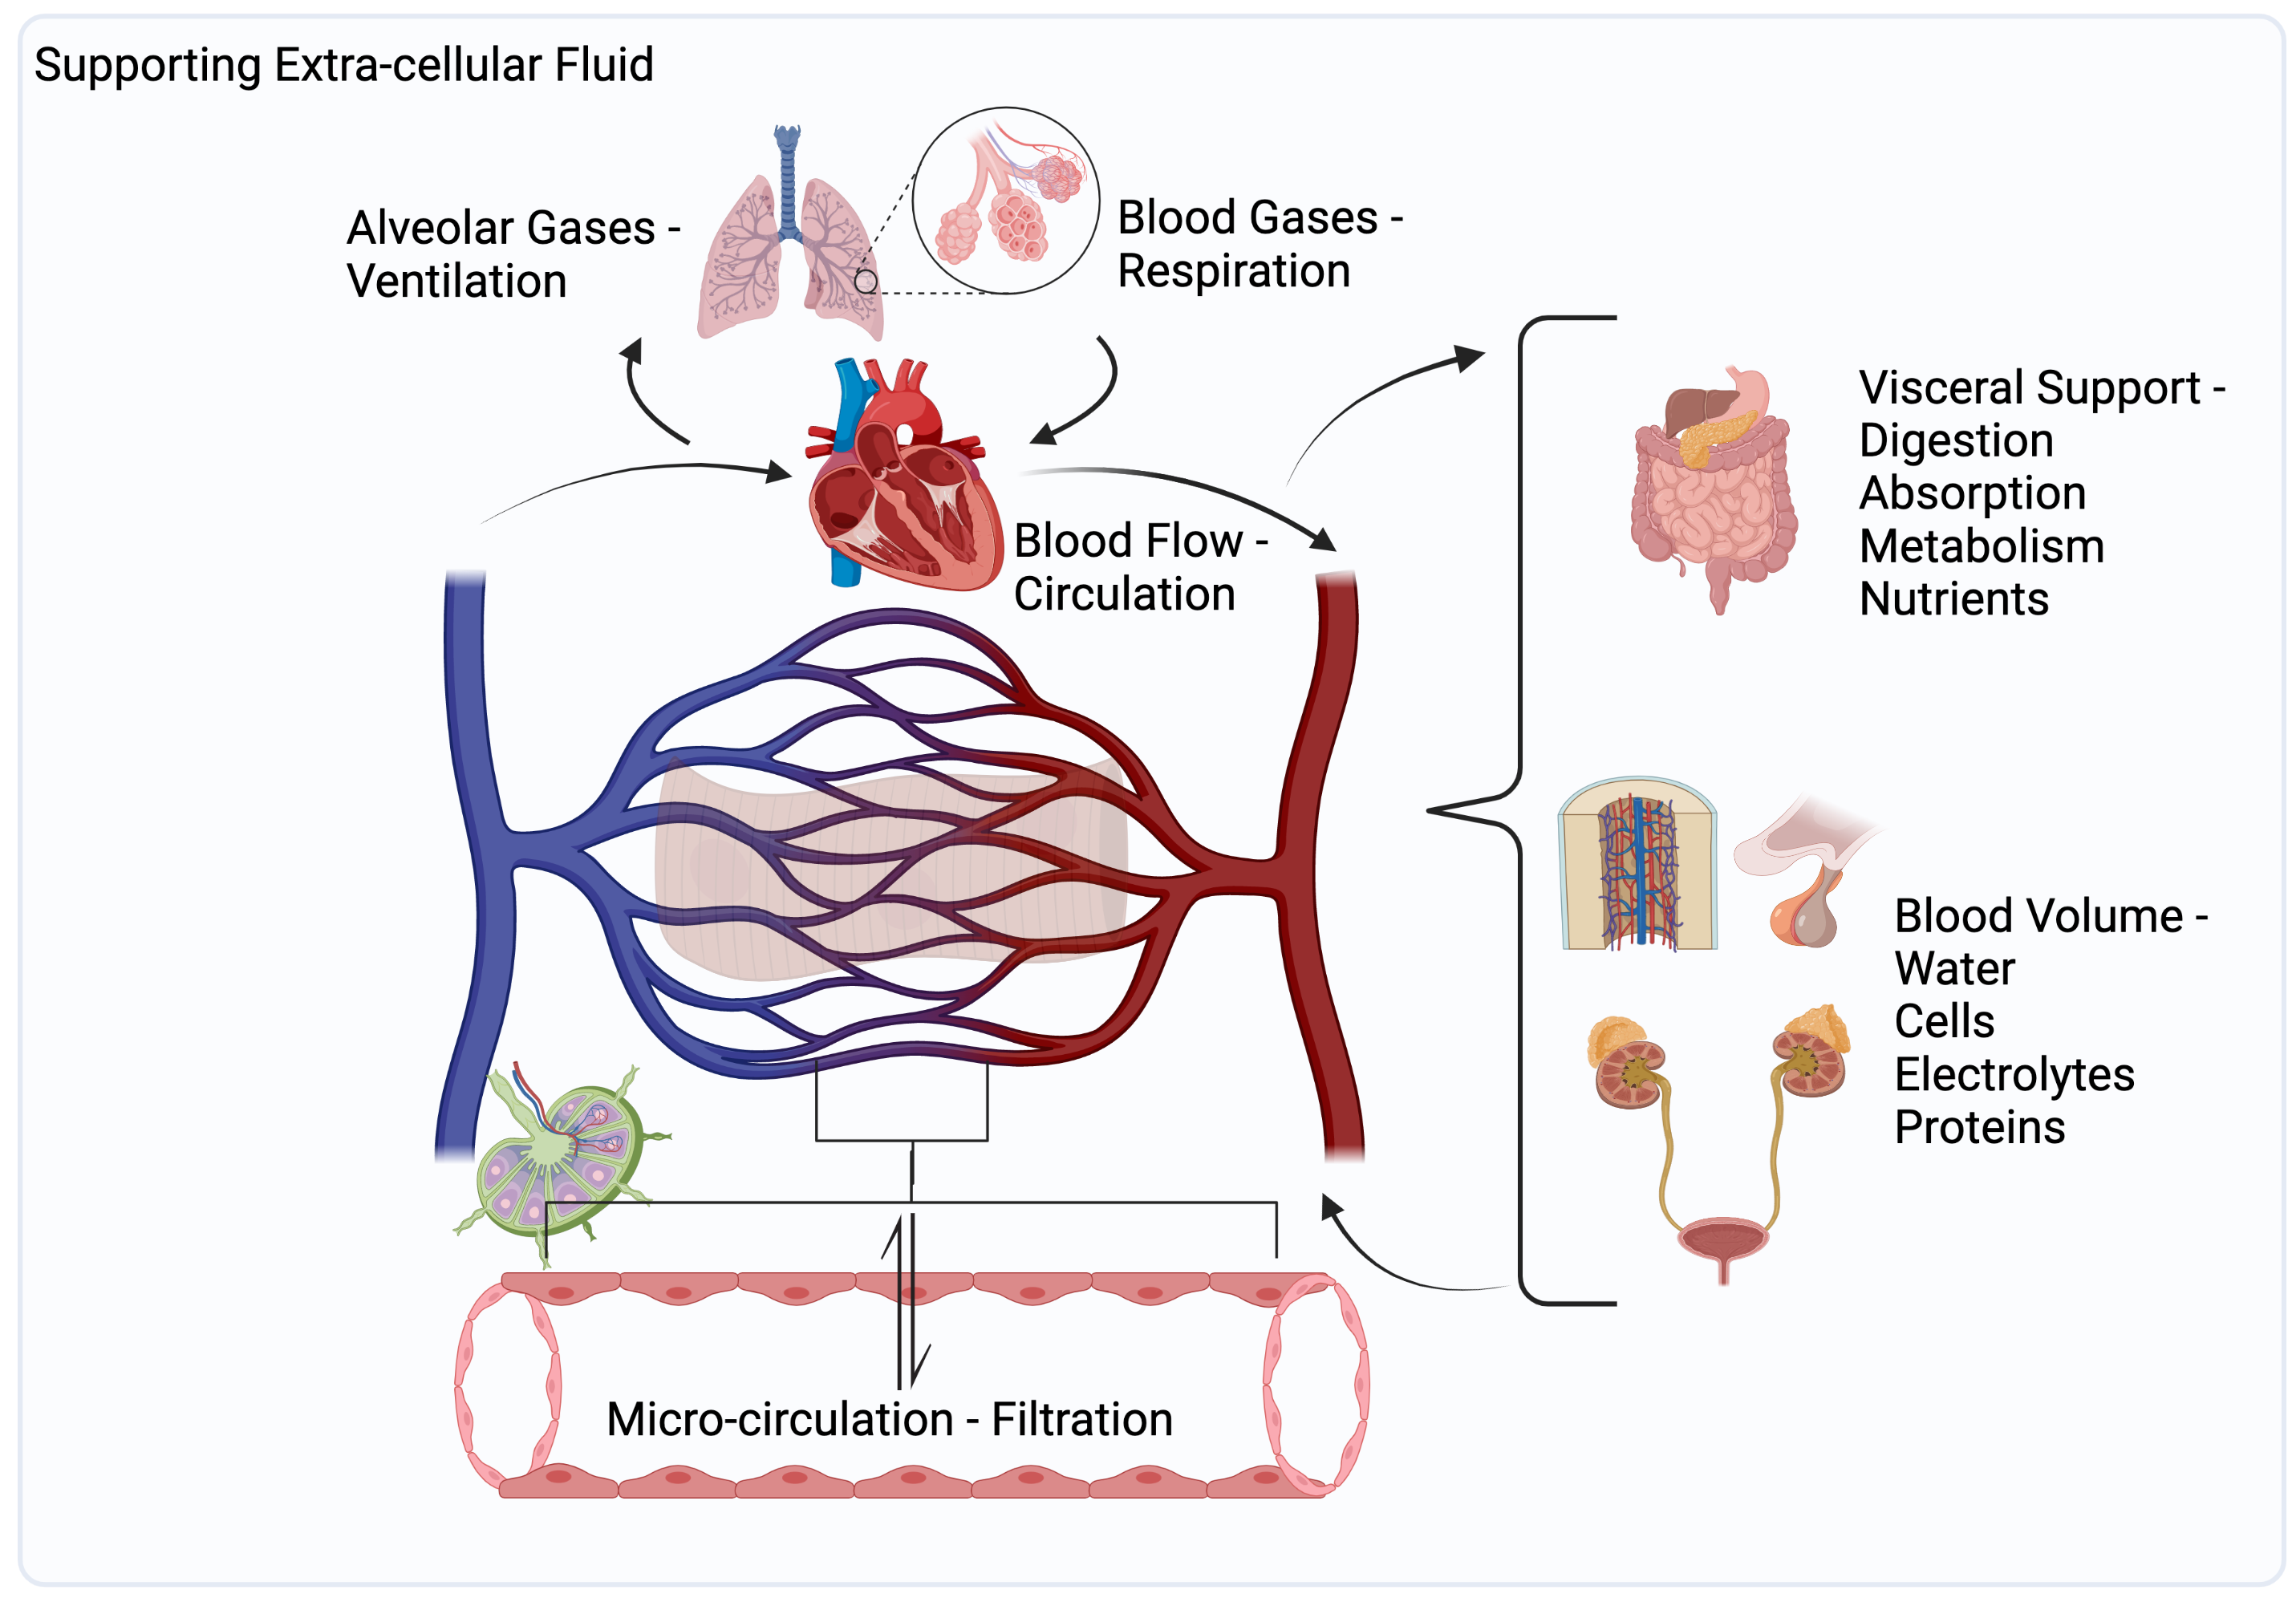
\includegraphics[width=1\linewidth]{./figure/part2_overview.png}
    \caption{Part II: Muscle Support Overview \footnotesize{Created with BioRender.com}}
    \label{fig:part2_overview}
\end{figure}

Together these systems support the ECF and therefore muscle fibers and muscle function. They maintain homeostasis of several important electrolytes (ions, including $H^+$ as measured by pH), nutrients, molecules, water and heat (temperature). They are integrated with several interactions and redundancies to provide support across a wide range of muscle demands in a wide range of circumstances, both good and bad.

\section{Micro Circulation}

The micro-circulation is the continuous movement of ions, nutrients and molecules between the blood plasma (vascular part of ECF) and interstitial fluid. Micro-circulation occurs through the semi permeable capillary membranes in a process called filtration. The capillary membranes allow relatively free passage of water, ions, molecules and  nutrients (other than proteins). The contents of plasma and interstitial fluid is similar other than cell and protein content (particularly red blood cells and albumin), which is limited due to an inability of these larger items to pass through the capillary membrane. There are also differences in $O_2$ and $CO_2$ due to the constant exchange with the cell.

Normal values of several important ions, molecules and nutrients are depicted in Figure \ref{fig:ecf}. Vascular and interstitial values are typically equal unless otherwise noted. $O_2$ and $CO_2$ pass easily through both the semipermeable capillary membrane and the semipermeable sarcolemma. There is a relatively large gradient for these molecules that varies due to the muscle fiber energetics. Normal function of circulation, respiration and ventilation at sea level are capable of equilibrating the vascular $O_2$ and $CO_2$ content even extreme high energetic situations.

\begin{figure}[!h]
    \centering
    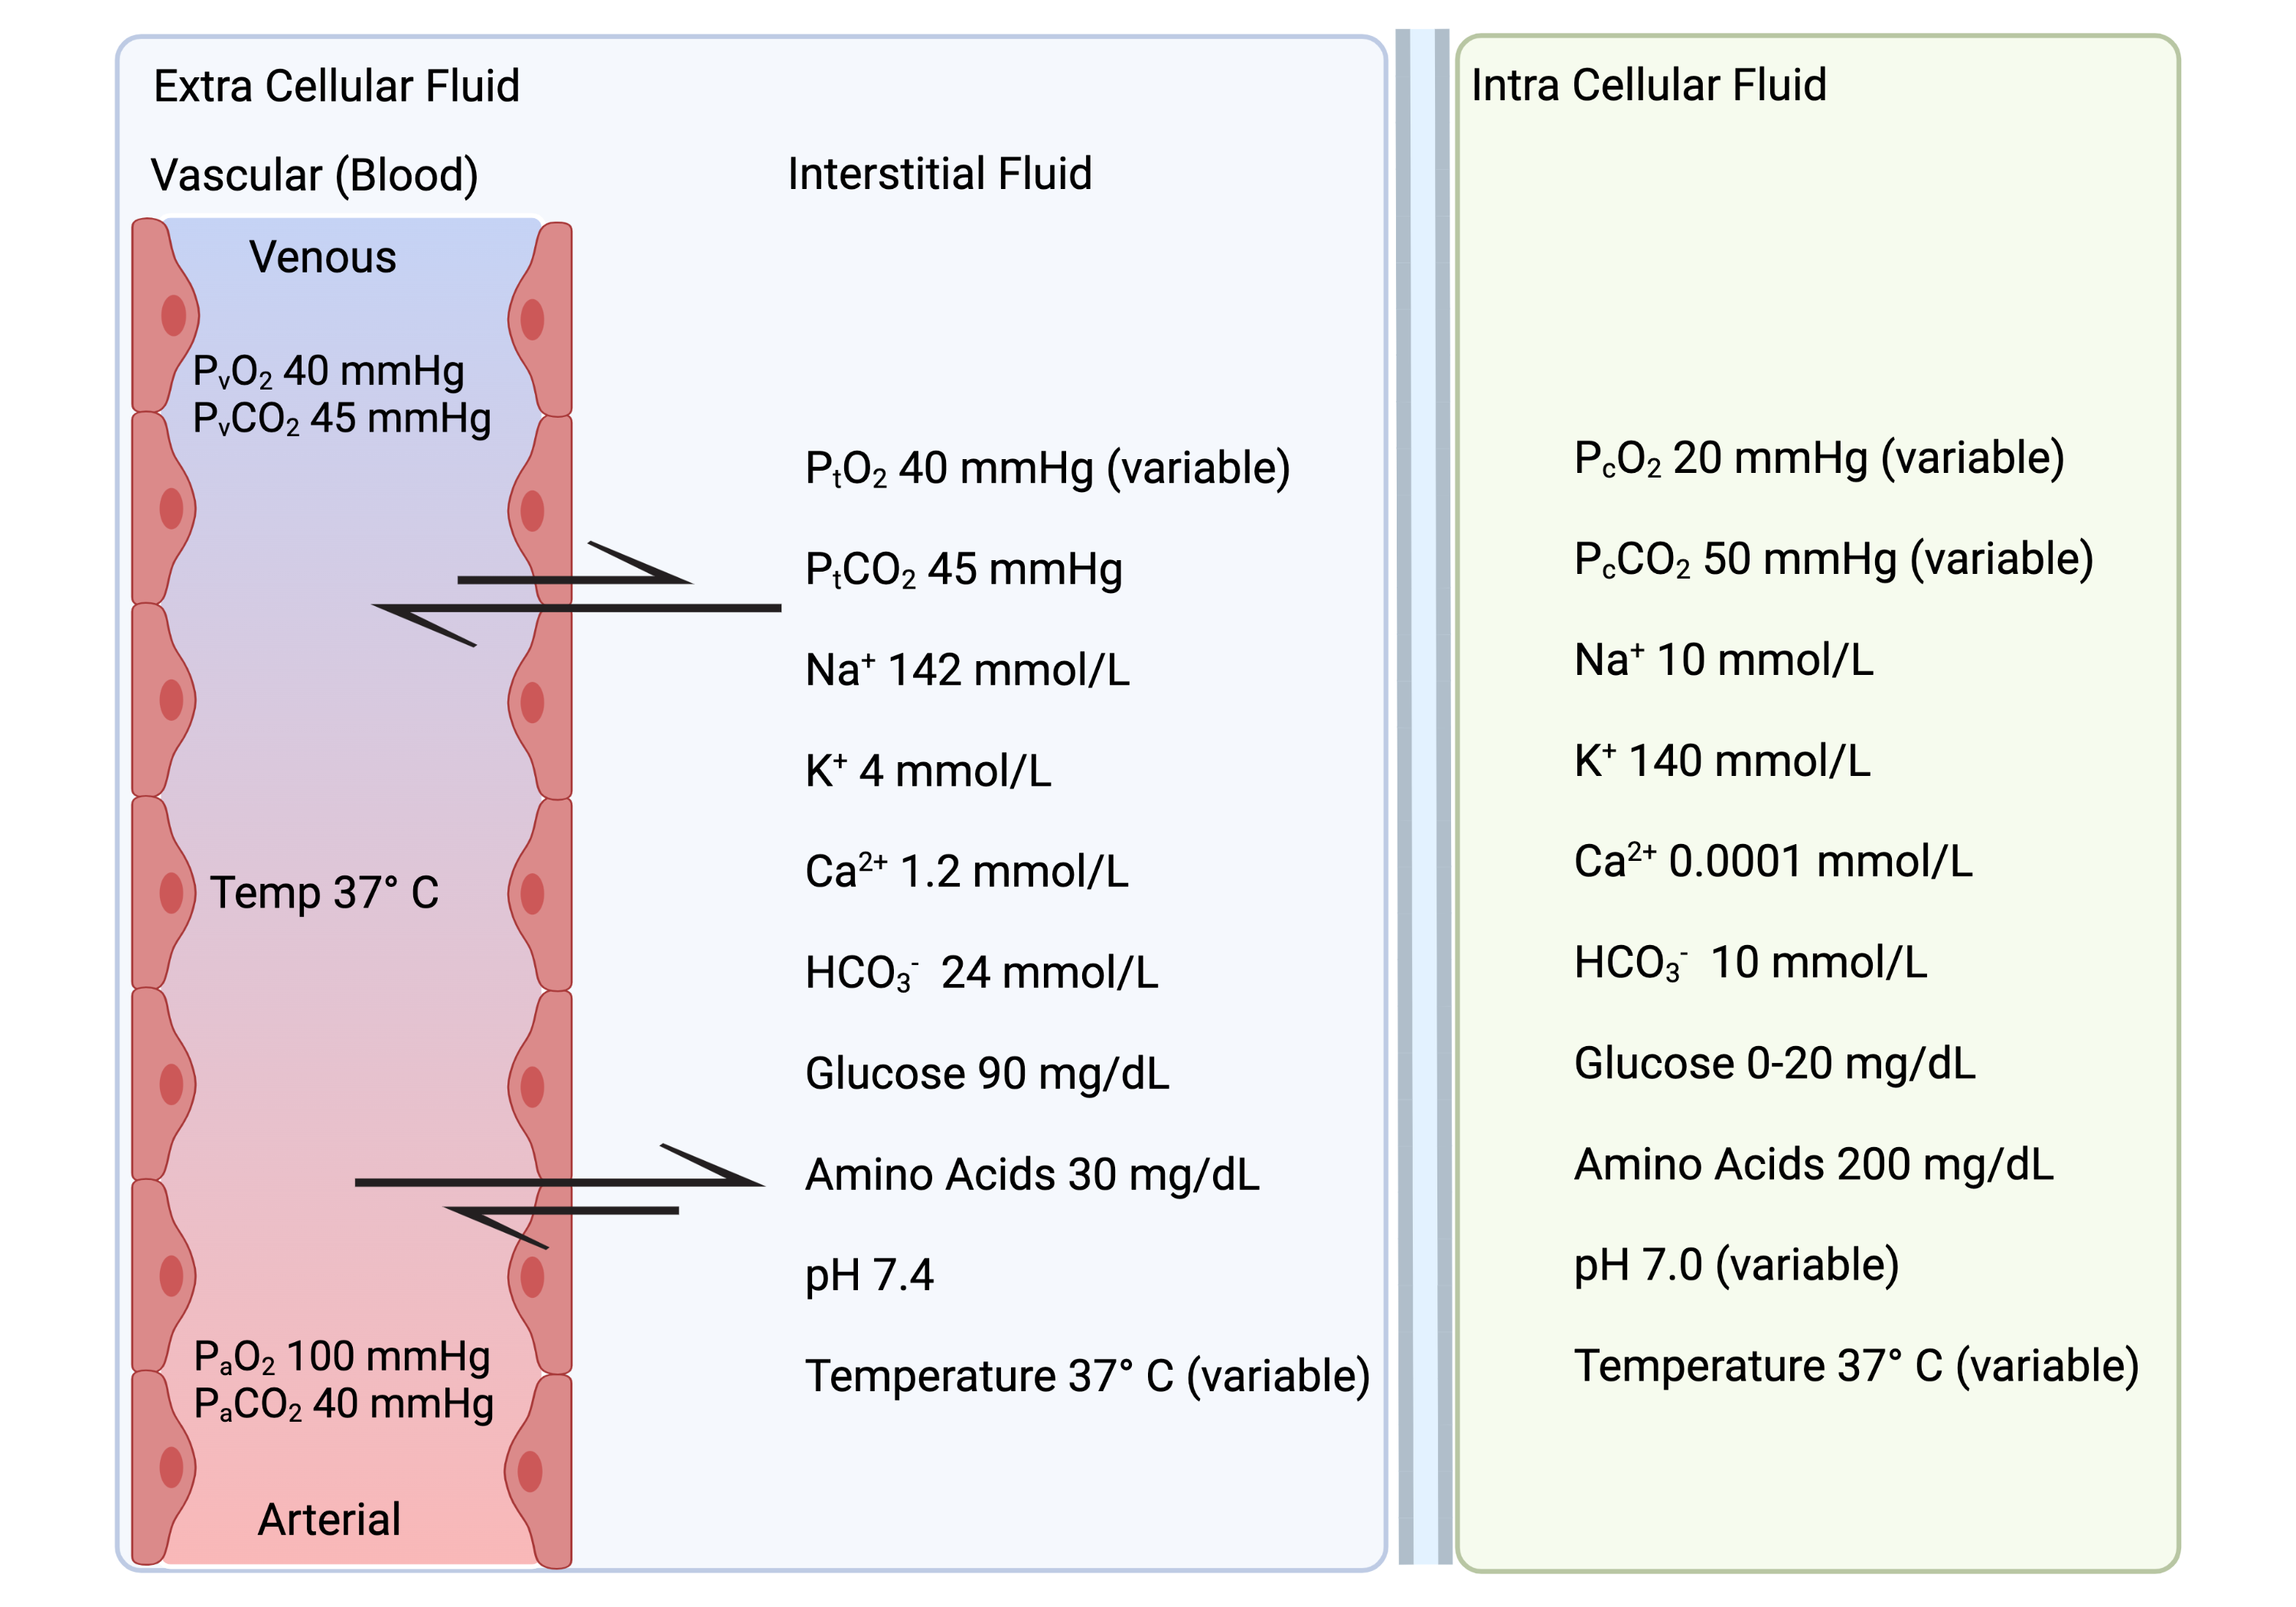
\includegraphics[width=1\linewidth]{./figure/ecf.png}
    \caption{Extra-cellular (Vascular \& Interstitial) and Intra-cellular Fluid \footnotesize{Created with BioRender.com}}
    \label{fig:ecf}
\end{figure}

\subsection{Extra Cellular - Intra Cellular Fluid Movement}

Exchange between the interstitial fluid and intracellular fluid occurs through the semi permeable cell membrane (sarcolemma). The sarcolemma restricts movements of ions and even with changes in the permeability for $Na^+$ and $K^+$ during excitation does not change the concentration difference between the interstitial and ICF fluid for these ions (at least under normal circumstances). The sarcolemma regulates the movement of nutrients.  Glucose uptake by a cell is influenced by the activation of the glut4 receptor channel for glucose by insulin. 

Between 50-70\% of an adult body is water. The variation in the percent of the adult body that is water is based on variations in lean (mostly muscle) tissue. In individuals with more muscle (particularly compared to adipose tissue) there is a higher percent of water. Of the total body water approximately 2/3 is intracellular (ICF) and 1/3 is extra cellular (ECF). Since water moves freely between the interstitial and ICF due to a large quantity of aquaporins (water channels) in the membrane the balance of ICF and ECF water volume is based largely on solute concentrations and resultant balance of osmotic pressure.

\subsubsection{ECF - ICF Water Volume Balance}

The sarcolemma is permeable to water but not to the ions. The osmolarity between the ECF and ICF determines whether there is net water movement by osmosis and the water (fluid) volume shifts between ECF and ICF. Under steady state conditions the osmolarity between the ECF and ICF is equal. Changes in solute concentration (ions, molecules, nutrients) in the ECF and ICF changes the osmolarity and results in movement of water until osmolarity balance is achieved.

\paragraph{Review of Osmotic Pressure}

At this point most people benefit from a review of these terms and the associated process of osmosis and osmotic pressure. Osmosis is the net movement of water across a selectively permeable membrane caused by a concentration difference across the membrane. Osmotic pressure is the pressure required to prevent osmosis of water through a membrane that is permeable to water but not to the solute (similar concept to an equilibrium potential). The osmotic pressure is an indication of how quickly osmosis will occur (driving force); and osmosis will not occur if there is no osmotic pressure. Osmotic pressure is exerted by particles and is determined by the number of particles per unit volume of fluid. 

The osmole (Osm) expresses solute concentration in terms of the number of particles. An Osm is the number of moles of solute that contribute to the osmotic pressure of a solution. Osmolarity refers to the number of osmoles in a volume (L) of solvent. Osmolarlity = Osm / Liter. Osmolarity is proportional to the milli osmoles / L as well (mOsm/L).

Osmotic pressure ($\pi$) is directly proportional osmolarity (concentration in Osm in a volume (L) of solvent) ($C$); the ideal gas constant ($R$); and absolute temperature ($K = 310^{\circ}$ at body temperature) in the equation: $\pi = C \cdot R \cdot T$. Since $R$ is a constant, and $K$ in the body is held constant, the osmotic pressure is determined by the osmolarity (Osm/L). At body temperature each 1 mOsm/L (milli osmole per liter) results in approximately 19.3 mmHg of osmotic pressure. In Figure \ref{fig:osmotic_pressure} the solution on the left has 1 mOsm/L more osmolarity. At body temperature this means 19.3 mmHg of pressure is required to stop the movement of water. Differences in osmolarity due to differences in solute concentration across the sarcolemma results in osmosis of water until there are no differences in osmolarity.

\begin{figure}[!h]
    \centering
    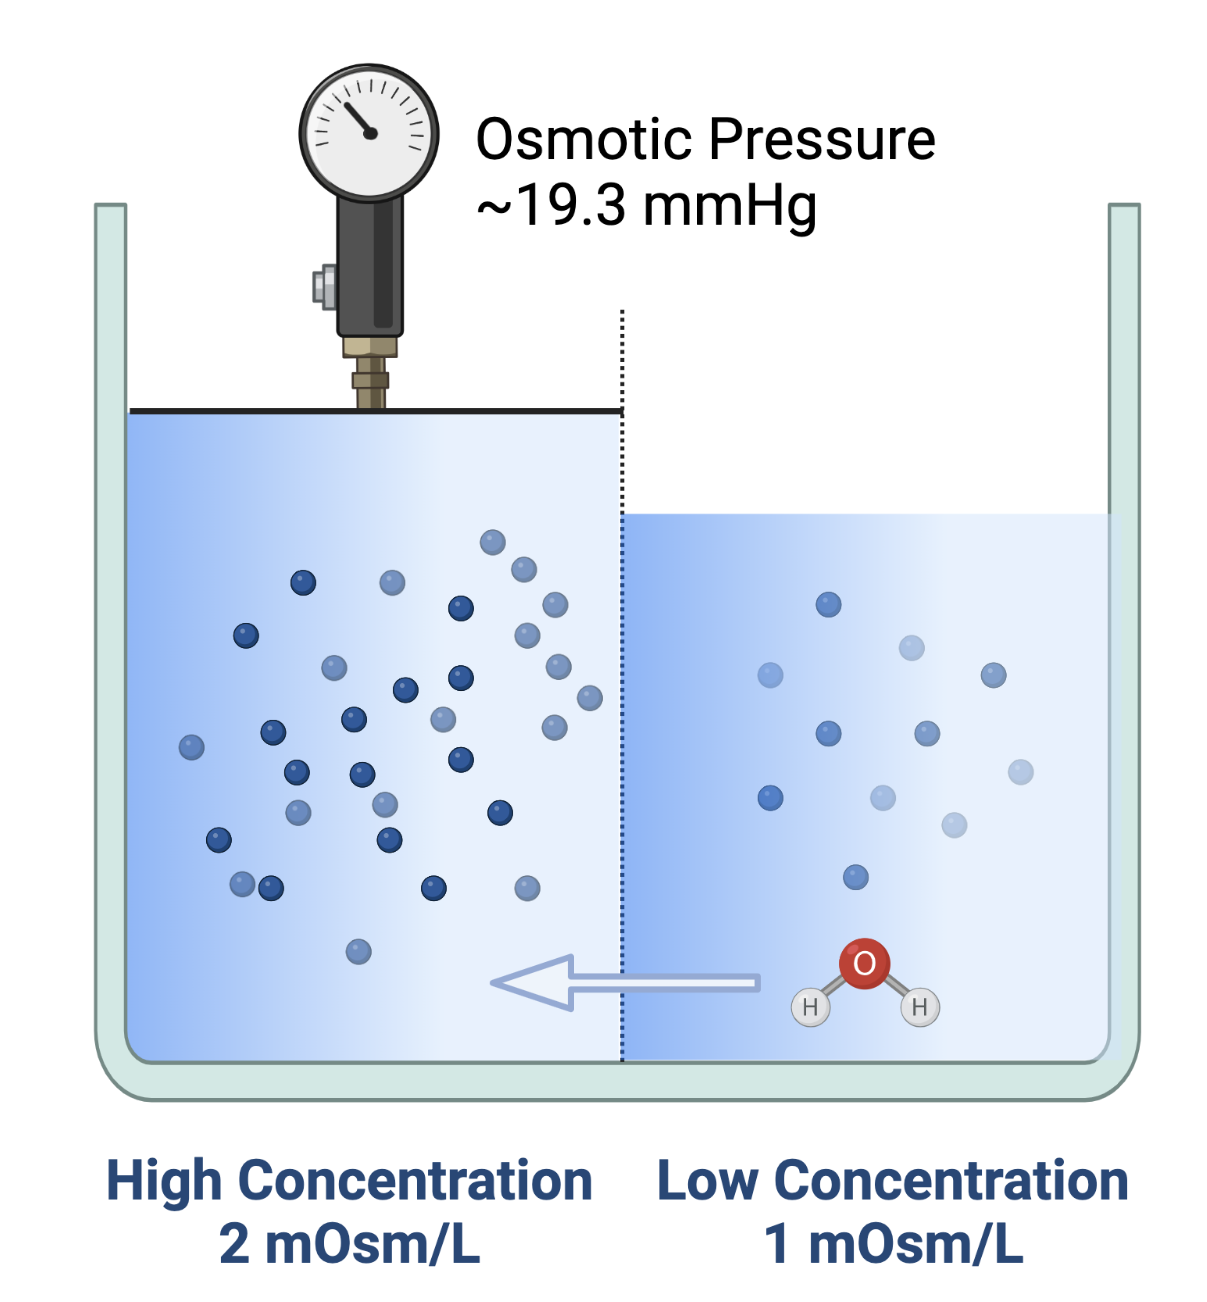
\includegraphics[width=1\linewidth]{./figure/osmotic_pressure.png}
    \caption{Osmotic Pressure \footnotesize{Created with BioRender.com}}
    \label{fig:osmotic_pressure}
\end{figure}

Since water moves freely across the sarcolemma osmosis occurs and balances the osmolarity of the ICF with that of the ECF. The osmolarity of ECF and ICF are equal and therefore there is no osmosis or net movement of water across the membrane since the osmotic pressures cancel each other out.

The total intake of water and ions (electrolytes) are carefully matched by equal outputs from the body to prevent fluid volumes and ion concentrations from fluctuating beyond acceptable ranges (mass balance, and homeostasis). There are times when there are differences between intake and output of water and ions that eventually must be remedied. Small shifts in water between ECF and ICF ensure that both compartments have the water required and maintain appropriate ion concentrations.

These shifts typically start with changes to the ECF. It is usually the ECF that we are adding water and ions to (ingestion, absorption). Water and ions are also removed from ECF in the kidneys, the colon (small amount under normal circumstances) and water is removed from ventilation.  These changes in water volume change the concentration and therefore osmolarity of ECF. Since all things that enter the ICF do so from the ECF the ICF does not typically have changes to osmolarity that are not provoked by the ECF first. There are some circumstances discussed below that ICF osmolarity may change in response to abnormalities in ICF $K^+$ concentration. 

The response to changes in osmolarity between the ECF and ICF is movement of water by osmosis until there is once again equalize the osmolarity. Large water intakes to the ECF such as large water intake or IV infusions; or decreases (dehydration) associated with sweating, GI fluid loss, or excessive urine formation by the kidneys (i.e. in diabetes mellitus) change the ECF water volume. If these changes alter the osmolarity of the ECF then water will pass between ECF and ICF until osmolarity is equalized.

Figure \ref{fig:iso_hypo_hypertonic} depicts the changes that would occur to the osmolarity with the addition of a volume of isotonic (same osmolarity), hypotonic (lower osmolarity), and hypertonic (higher osmolarity) solution to the ECF.

\begin{figure}[!h]
    \centering
    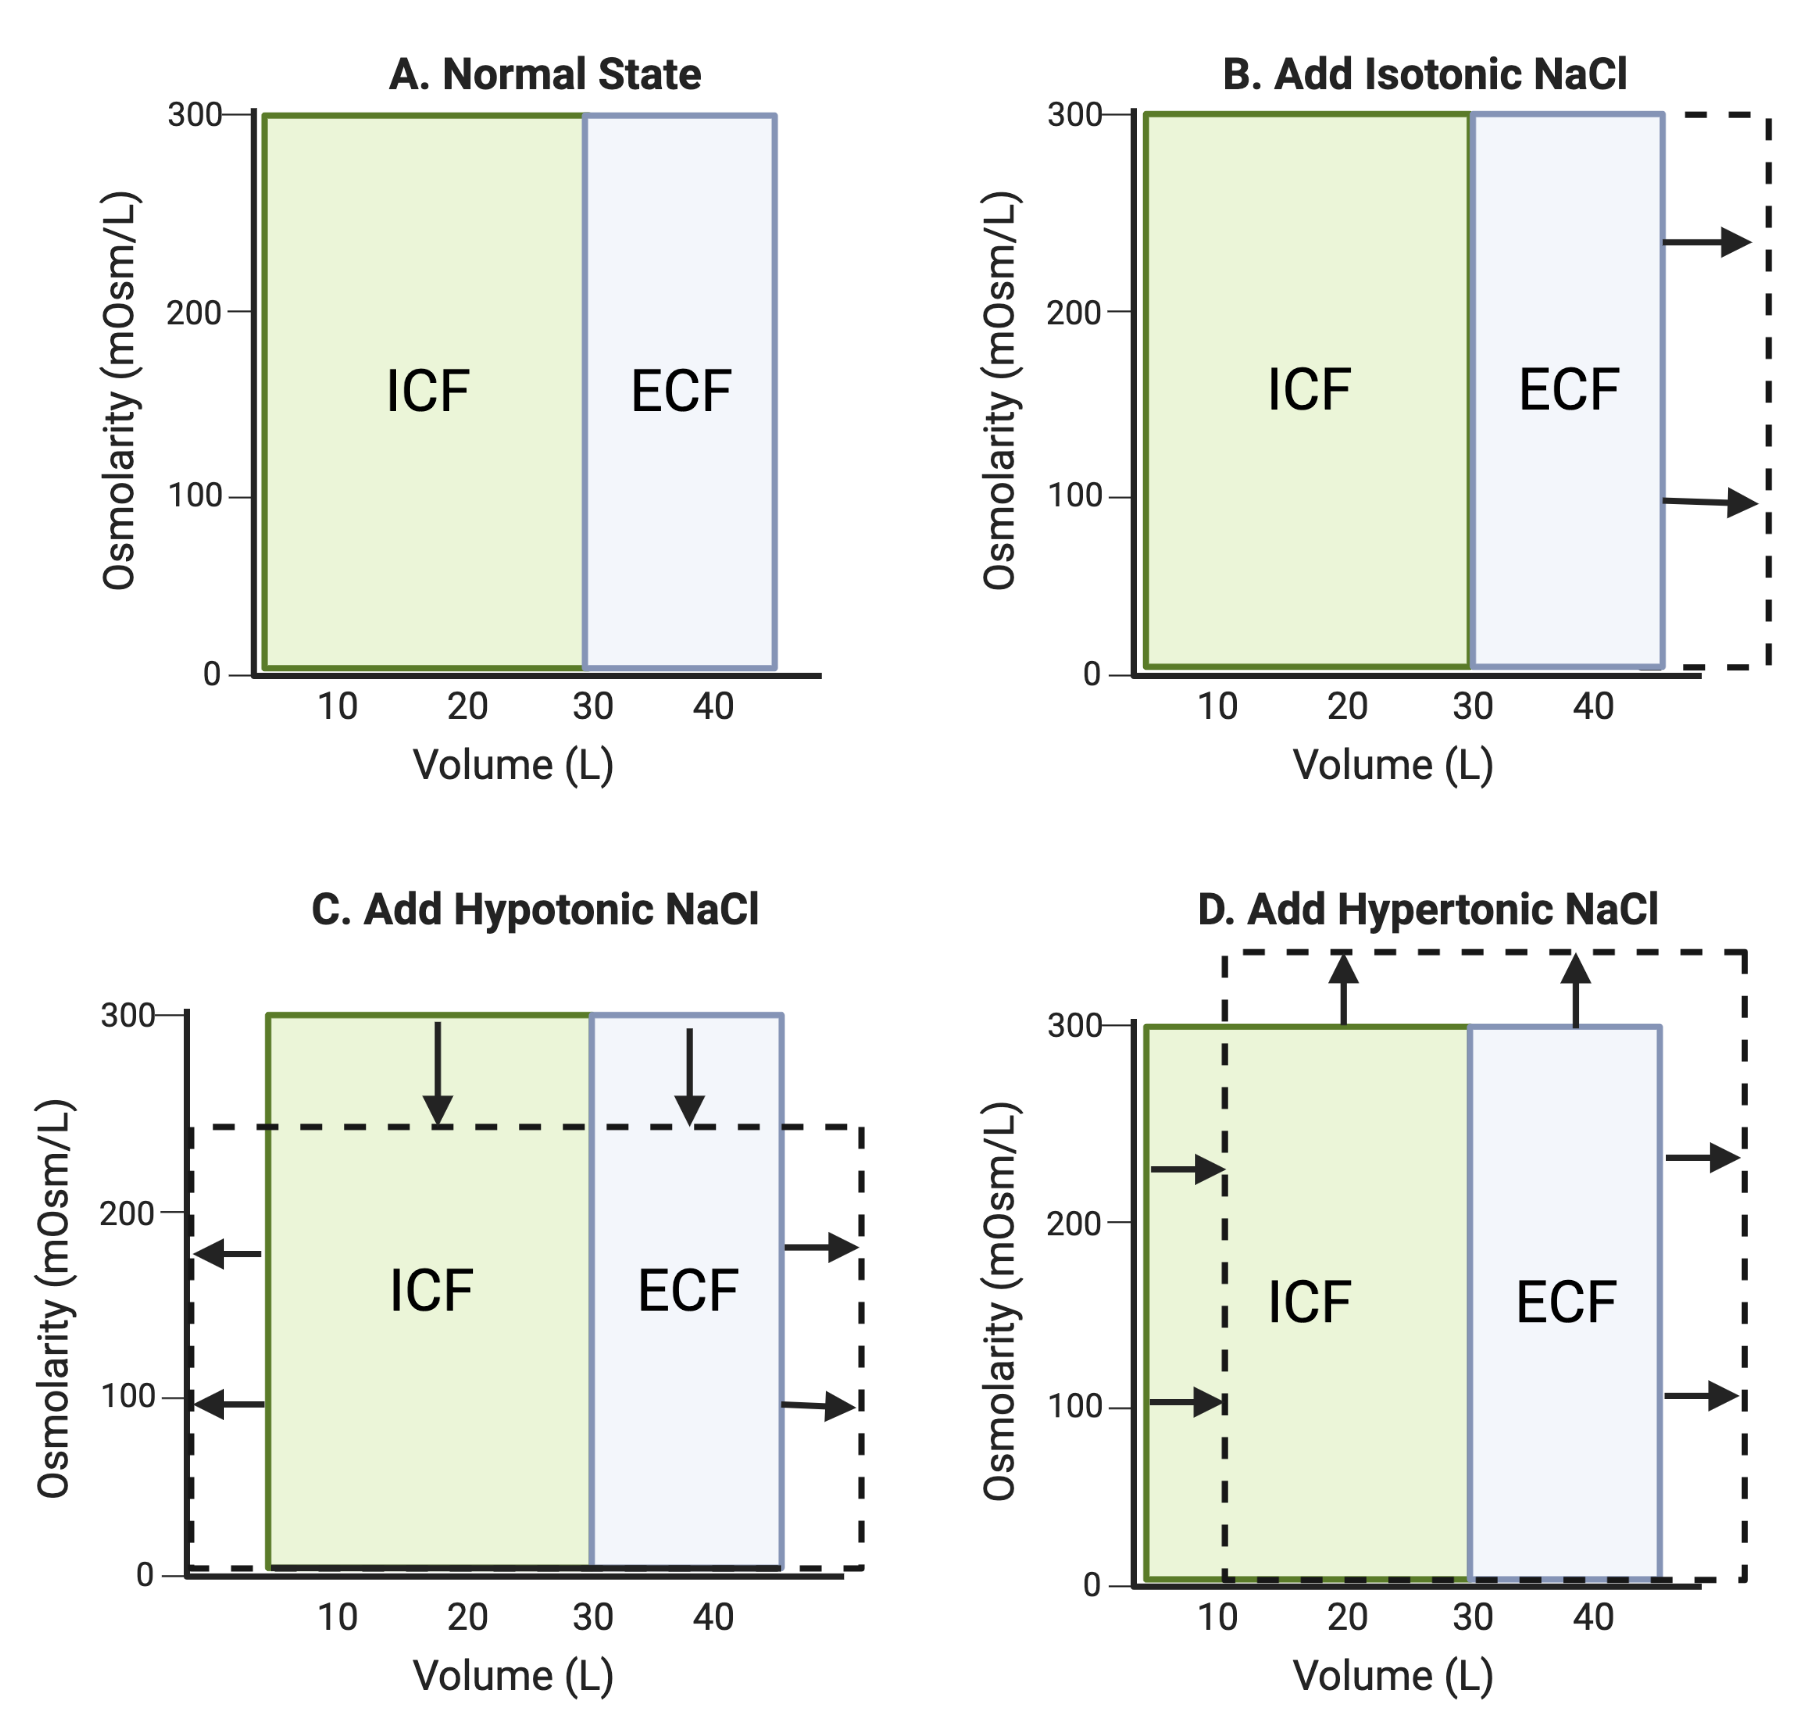
\includegraphics[width=1\linewidth]{./figure/iso_hypo_hypertonic.png}
    \caption{Impact of ECF Infusions of Iso, Hypo and Hypertonic Solutions (See text for details) \footnotesize{Created with BioRender.com}}
    \label{fig:iso_hypo_hypertonic}
\end{figure}


\begin{itemize}
    \item Adding an isotonic solution to ECF does not change osmolarity of the ECF so there is no osmosis (no change in net water movement). The end result is an increase in ECF volume but no change to ICF volume (See Figure \ref{fig:iso_hypo_hypertonic} B).
    \item Adding a hypotonic solution to ECF decreases the osmolarity of ECF and results in osmosis of water into the cells (ICF) and increases ICF volume. This continues until the osmolarity of ICF decreases and the concentration of ECF increases until the osmolarity of both compartments are equal which stops the net flow of water into the ICF. The overall effect is increased ICF and ECF volume, and decreased ICF and ECF osmolarity (See Figure \ref{fig:iso_hypo_hypertonic} C). 
    
    % Stopped here.......
    
    \item Adding a hypertonic solution to ECF increases the osmolarity of ECF and results in osmosis of water out of the cells (ICF) and decreases ICF volume. This continues until the osmolarity of ICF increases and osmolarity of both compartments are equal which stops the net flow of water out of the ICF. The overall effect is decreased ICF volume and increased ECF volume; and an increase of osmolarity of both ICF and ECF.
\end{itemize}

\paragraph{Importance of Osmosis to Muscle Excitation}

An important connection to make is that changes in the osmolarity of the ECF and ICF is based on the concentration of these solutions. The concentration changes with changes to the water volume or changes to the amount of solute. A hypertonic solution therefore increases the concentration of $Na^+$ in both the ECF and ICF, but retains the concentration gradient. A hypotonic solution decreases the concentration of $Na^+$ in the ECF and ICF, but does not change the concentration gradient. Since the concentration gradient of $Na^+$ (and all ions) across the sarcolemma is critical to excitation, it should be clear that these osmotic pressure directed fluctuations to water volume serve an important buffer capacity to maintain these ion concentration gradients. Dehydration, a reduction in water volume, ultimately results in a slightly higher concentration of ions, but this higher concentration is balanced between the ECF and the ICF, so gradients are kept constant.
Ion abnormalities exist (electrolyte imbalances), but they do not have as profound an impact as they would if water did not move freely between ECF and ICF to normalize concentration gradients. 

\subsection{Extra cellular Values \& Ranges}

Table \ref{table:ecf_value_ranges} provides normal values and ranges and non lethal limits for several important components of the ECF.  The wide normal ranges and non lethal limit ranges is a good example of the degree of overall robustness. Moving outside of a range without an easy temporary explanation (such as low $P_v O_2$ in response to exercise) is an indication that something is wrong. But even when something is wrong, the body adjusts and even large deviations in normal values are tolerated before the changes become lethal. Several of these components of the ECF have larger non lethal limits in one direction. For example, $P_v O_2$ can increase tremendously (if given a large amount of oxygen in hyperbaric (high pressure) systems) before it becomes lethal. The criteria for lethal for these values is death. Some of the secondary effects may lead to premature death. 

\begin{table}[h!]
\centering
\begin{tabular}{||c c c c||} 
 \hline
Value & Normal Value & Range & Non-Lethal Limit\\ [0.5ex] 
 \hline\hline
 $P_v O_2$ (mmHg) & 40  & 25-40 & 10-1000 \\
 $P_v CO_2$ (mmHg) & 45 & 41-51 & 5 - 80\\ 
 $Na^+$ (mmol/L) & 142 & 135 - 145 & 115 - 175\\
 $K^+$  (mmol/L) & 4.2 & 3.5 - 5.3 & 1.5 - 9.0\\ 
 $Ca^{2+}$ (mmol/L) & 1.2 & 1.0 - 1.4 & 0.5 - 2.0 \\
 $HCO_3 ^-$ (mmol/L)& 24 & 22 - 29 & 8 - 45 \\
 Glucose (mg/dL)& 90 & 70 - 115 & 20 - 1500 \\
 Acid-Base (pH) & 7.4 & 7.3 - 7.5 & 6.9 - 8.0 \\
 Temperature F (C) & 98.6 (37) & 98-98.8 (37) & 65-110 (18.3-43.3)[1ex] 
 \hline
\end{tabular}
\caption{Normal Range and Non Lethal Limits of Values in ECF (\footnotesize{Data from \cite{feher_quantitative_2017}})}
\label{table:ecf_value_ranges}
\end{table}

For example, while a $Na^+$ value of 165 mmol/L is within the non lethal limit. This concentration of $Na^+$ is buffered by the movement of water that would occur due to changes in the osmolarity of the ECF so its impact on the concentration is not as great as it may seem. But with such a high concentration it would be associated with, amongst other signs and symptoms of hypernatremia, a high blood volume and therefore high blood pressure despite attempts to maintain normal blood pressure. The elevated blood pressure can then lead to premature death.  Tolerance for temperature is greater with cold than with heat. With heat proteins denature and metabolic functions cannot be catalyzed. With decreased temperature reactions slow down from reduced kinetic energy, but at least the enzymes (proteins) are functioning. 


\subsection{Oxygen \& Carbon Dioxide}

The gradient for $O_2$ from the vascular fluid into the cell exists because the cell is constantly utilizing $O_2$. The gradient for $CO_2$ from the cell to the vascular fluid exists since the cell is constantly producing $CO_2$. The other gradient for $O_2$ and $CO_2$ depicted in Figure \ref{fig:ecf} is from the arterial end of the capillary to the venous end of the capillary. As shown, with healthy capillaries, normal capillary blood flow and normal blood the vascular $O_2$ and $CO_2$ partial pressure equilibrate by the time blood reaches the venous end of the capillary. The cellular and interstitial partial pressure for oxygen ($P_c O_2$ \& $P_t O_2$) are variable based on how much $O_2$ is being consumed in the muscle fiber, which is dependent on the rate of ATP regeneration occurring in electron transport (ETC). With a higher than resting ATP regeneration in ETC the $P_c O_2$ will drop, which drops the $P_t O_2$ below 40 mmHg, and then the partial pressure of oxygen at the venous end $P_v O_2$ of the capillary will also drop. $P_v O_2$ will equilibrate to $P_t O_2$. However, the $P_a O_2$ will remain at 100 mmHg as long as the circulation and pulmonary systems are providing the additional support that is required.

Similarly, for ETC to be regenerating ATP at a higher rate, TCA has to be functioning at a higher rate and thus producing more $CO_2$. This results in a higher $P_c CO_2$. However, because $P_t CO_2$ and $P_v CO_2$ equilibrate, as long as the circulation and pulmonary systems are providing the additional support that is required there will not be an increase in either $P_t CO_2$ or $P_v CO_2$. The difference between arterial $O_2$ and venous $O_2$ is an important indicator of how much $O_2$ is being consumed. How much $O_2$ is being consumed is an indicator of metabolism and energetic demands from rest to peak exercise. This relationship is captured in the Fick Equation discussed in Chapter \ref{chp:fick_equation}:

\begin{equation}
    \dot{V}O_2 = \dot{Q} \cdot (a-v)O_2
\end{equation}


\subsection{Temperature}

Temperature is heat unless there is a temperature of 0 degrees Kelvin. Heat is a byproduct of all energetic transformations, including regenerating ATP and hydrolyzing ATP. At rest, temperature in muscle fiber tends to equilibrate (or slightly lower) with that of the body because the flow of heat from the fibers into the ECF is moved to the blood and out of the region. Some of the heat also dissipates through the ECF and tissues across the temperature gradient directly out of the body. When core body temperature falls, a reflex action is to shiver, which utilizes muscle activity to generate more heat for sharing with the rest of the body through the transport of ECF. When muscle temperature rises during activity, the circulation of blood carries much of that heat away from the muscle for dissipation throughout the body. As heat rises, more of the circulation is sent to the skin to facilitate this process.
Temperature of muscles varies more than core temperature. While core temperature is highly regulated at 37 degrees celsius muscles in the extremities, and more so the distal extremities, can vary from as high as 40 degrees in a hot environment to as low as 20 degrees in the cold. Muscle function when muscle tension is less than 37 degrees impacts the rate of tension development and the rate of tension recovery (relaxation). At the extreme of 22 degrees a the rate of tension development and recovery is approximately 25\% of that at 37 degrees \cite{jones_skeletal_2006}. This is thought to be due primarily to the dependency on these rates on kinetic energy of moving molecules throughout the chain of events from excitation to activation. The overall impact is that reductions in muscle temperature has a greater impact on high power activities which are dependent on the rate of tension development and recovery.

\subsection{Acid Base (pH)}

Intra cellular fluid has several buffering systems for regulating pH through a wide range of energetic rates and thus do not, in resting or even low to moderate energetic situations, send $H^+$ ions out of the sarcoplasm for acid base balance. In high energetic circumstances, such as those discussed in Chapter \ref{chp:energetics} with the glygogen $\rightarrow$ lactate pathway, lactate (lactic acid) removes excessive $H^+$ ions from the sarcoplasm to the ECF which can then be circulated to other cells for recycling.
There are several processes involved with the regulation of ECF acid base balance (pH). Each is presented in the upcoming chapters such as buffers in the blood and through filtration in the kidneys (Chapter \ref{chp:blood_content}, and respiration (Chapter \ref{chp:blood_oxygen}.


\section{Filtration}

Micro-circulation relies on filtration between the ECF vascular and the interstitial compartments. Filtration occurs through capillary membranes. It includes the flow and exchange of water, ions, molecules and some nutrients (glucose, fatty acids, amino acids). As previously discussed, larger items such as proteins (albumin) and blood cells do not normally filtrate through the capillary membranes. However, in certain circumstances white blood cells, as part of an immune response, will leave the circulation and enter the interstitial fluid.

There are two flow gradients that drive filtration, osmotic pressure and hydrostatic pressure. Osmotic pressure, as previously discussed, drives the movement of water and solutes out of and then back into the vascular compartment. The osmolarity between the vascular fluid and interstitial fluid is one driving force for filtration. The second flow gradient is hydrostatic pressure (fluid pressure) is the force that the fluids exert on the walls of the space they are, and is related to the size of that space (volume) in and the compliance of the walls of that space. Pressure, volume and compliance are related by the equations (C = compliance, V = volume, P = pressure:

\begin{equation}
    C = \frac{\Delta V}{\Delta P}
    \frac{1}{\Delta P} = \frac{C}{\Delta V}
    \Delta P = \frac{\Delta V}{C}
\end{equation}

Compliance is determined by the response of pressure to changes in volume. However, it is useful to consider how changes in compliance influence pressure with the assumption of a stable volume, or the influence on volume with the assumption of a stable pressure.

The volume of capillaries are the sum of their cross sectional area. Their cross sectional area is determined by their radius. The radius also influences their resistance to flow. And their flow influences the amount of fluid entering and exiting. These relationships are complicated, in part, because the radius of the capillaries influences their pressure (by changing their cross sectional area and volume), and their resistance to flow. The effect of these relationships is that changing capillary radius has a powerful, and complicated, effect on hydrostatic pressure in the capillaries.


\subsection{Capillary Regulation of Filtration}

The capillaries are involved in the regulation of filtration. Changing the radius of the capillaries can change the volume of blood entering the capillaries and can change the hydrostatic pressure but many of these changes are quickly adjusted. For example, a reduction in capillary radius may initially increase the hydrostatic pressure, but it also reduces the amount of blood flowing to the capillary so that the hydrostatic pressure normalizes. If all capillaries simultaneously decreased their radius then there would not be a drop in blood flow and the hydrostatic pressure. 

Changes to the radius of arterioles and the use of pre-capillary sphincters regulates the flow of blood into the capillaries and therefore has, at least temporary ability to adjust hydrostatic pressure (Figure \ref{fig:capillaries}. These changes tend to regulate flow and a reduction in flow will quickly result in normalization of hydrostatic pressure.

\begin{figure}[!h]
    \centering
    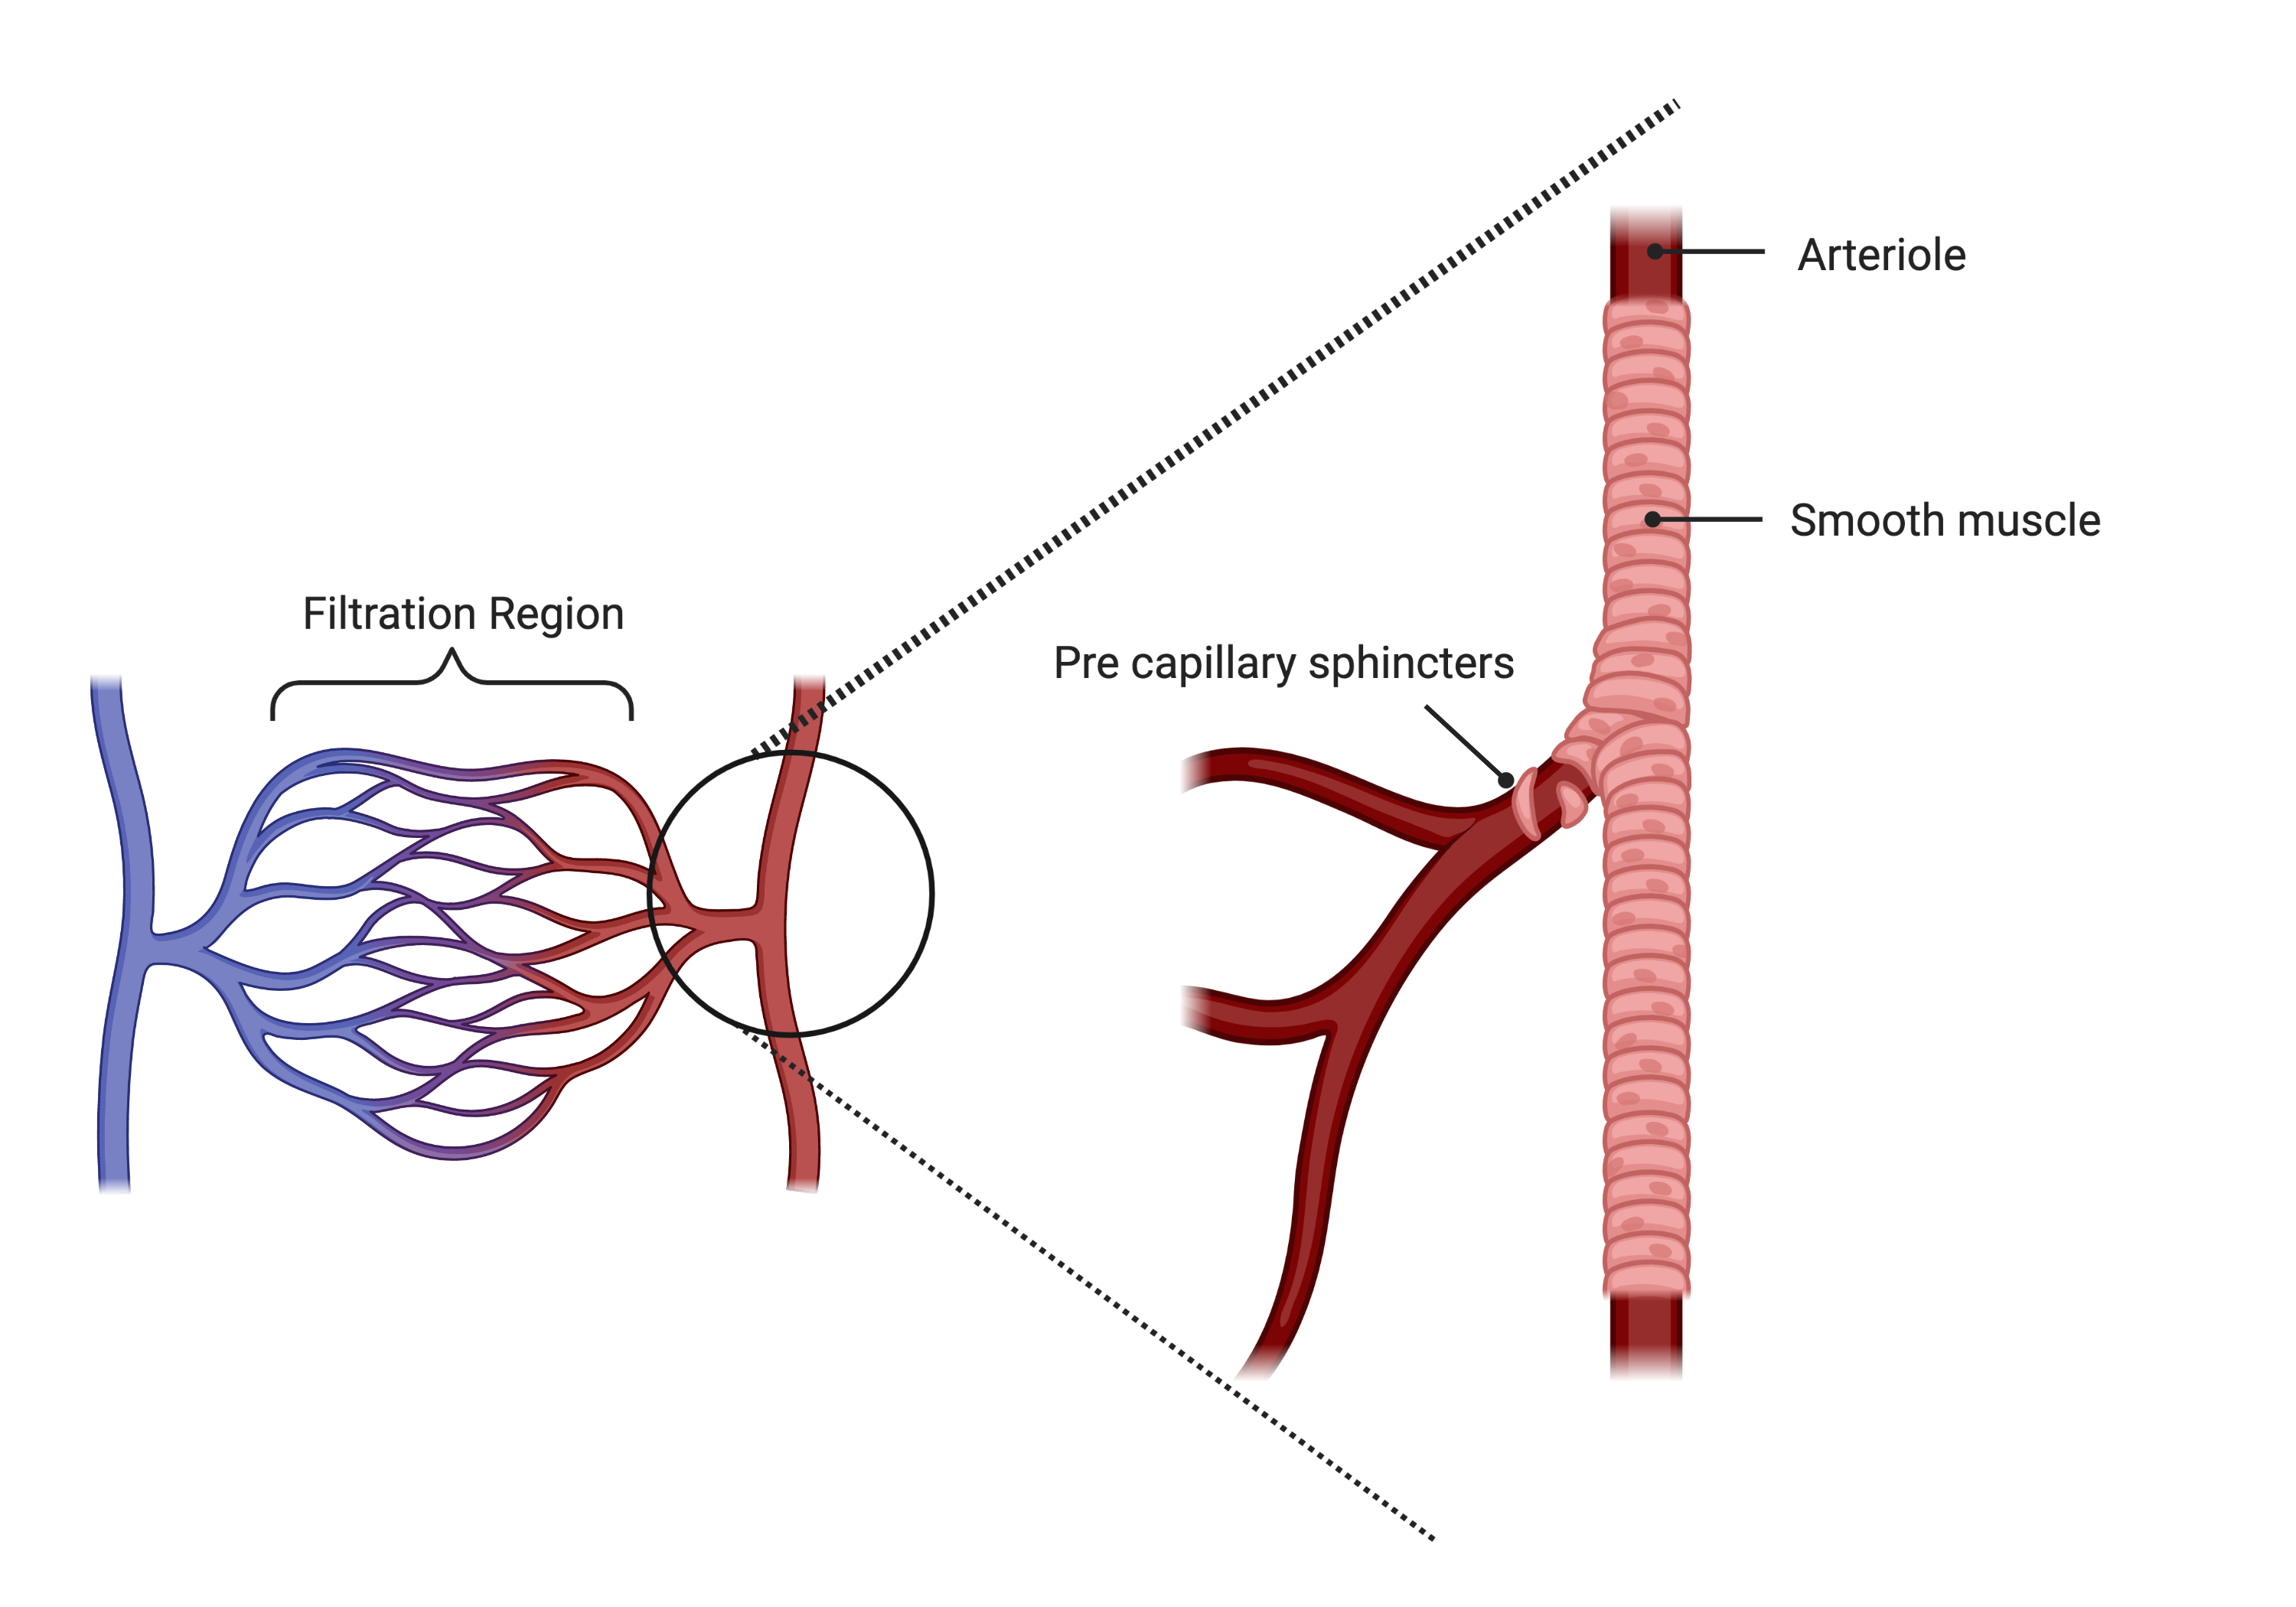
\includegraphics[width=1\linewidth]{./figure/capillaries.png}
    \caption{Capillary Anatomy \footnotesize{Created with BioRender.com}}
    \label{fig:capillaries}
\end{figure}


The capillary membrane can also change the size of its openings which can allow cells that could not previously leave the vascular compartment to enter the interstitial fluid. When this occurs, such as with capillary dilation in response to cellular inflammatory mediators or other threats to the well being of cells, the white blood cells enter the interstitial space and change the osmolarity and osmotic pressure gradients. 

\subsection{Filtration Pressures}

The overall filtration pressures (hydrostatic (P) and osmotic ($\pi$)) are just slightly unbalanced. This unbalance tends toward pushing fluid and solute out of the vascular compartment and into the interstitial compartment and leaving some of the fluid and solute in the interstitial compartment. The volume of fluid and solute left in the interstitial compartment then enters the lymphatic system and reenters the vascular system after circulation and filtration through the lymph vessels and nodes. 
The equation for filtration is depicted in Figure \ref{fig:filtration_equation}. 

\begin{figure}[!h]
    \centering
    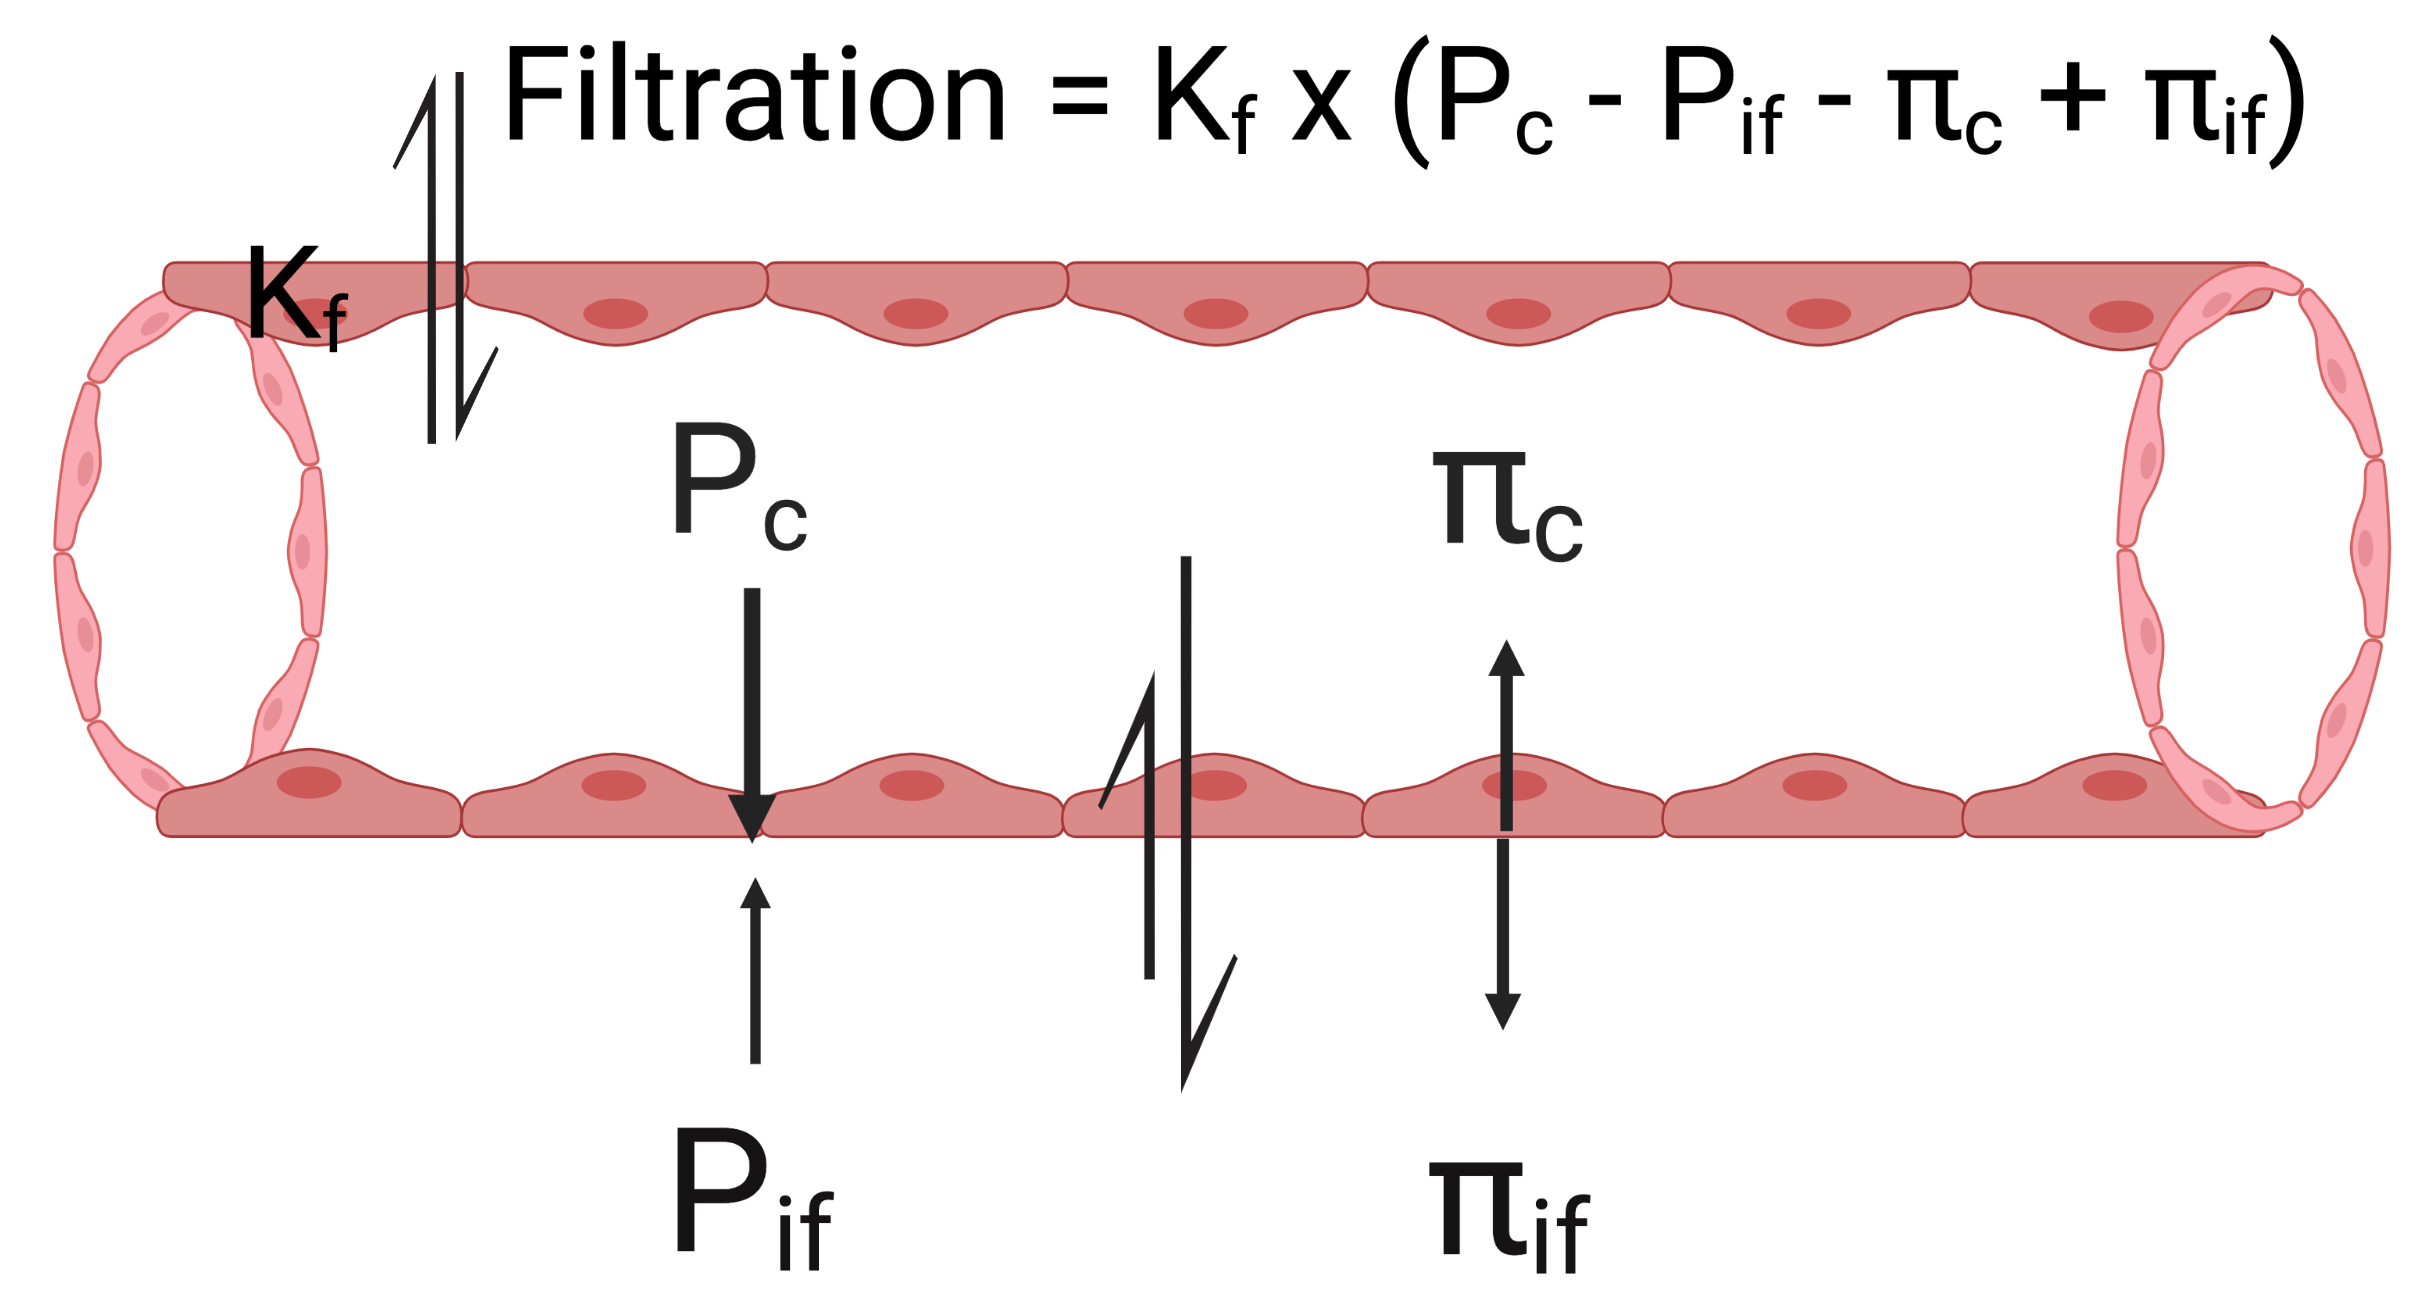
\includegraphics[width=1\linewidth]{./figure/filtration_equation.png}
    \caption{Filtration Equation Anatomy \footnotesize{Created with BioRender.com}}
    \label{fig:filtration_equation}
\end{figure}

\subsection{Micro-circulation Regulation}

\subsection{}
\begin{figure}[!h]
    \centering
    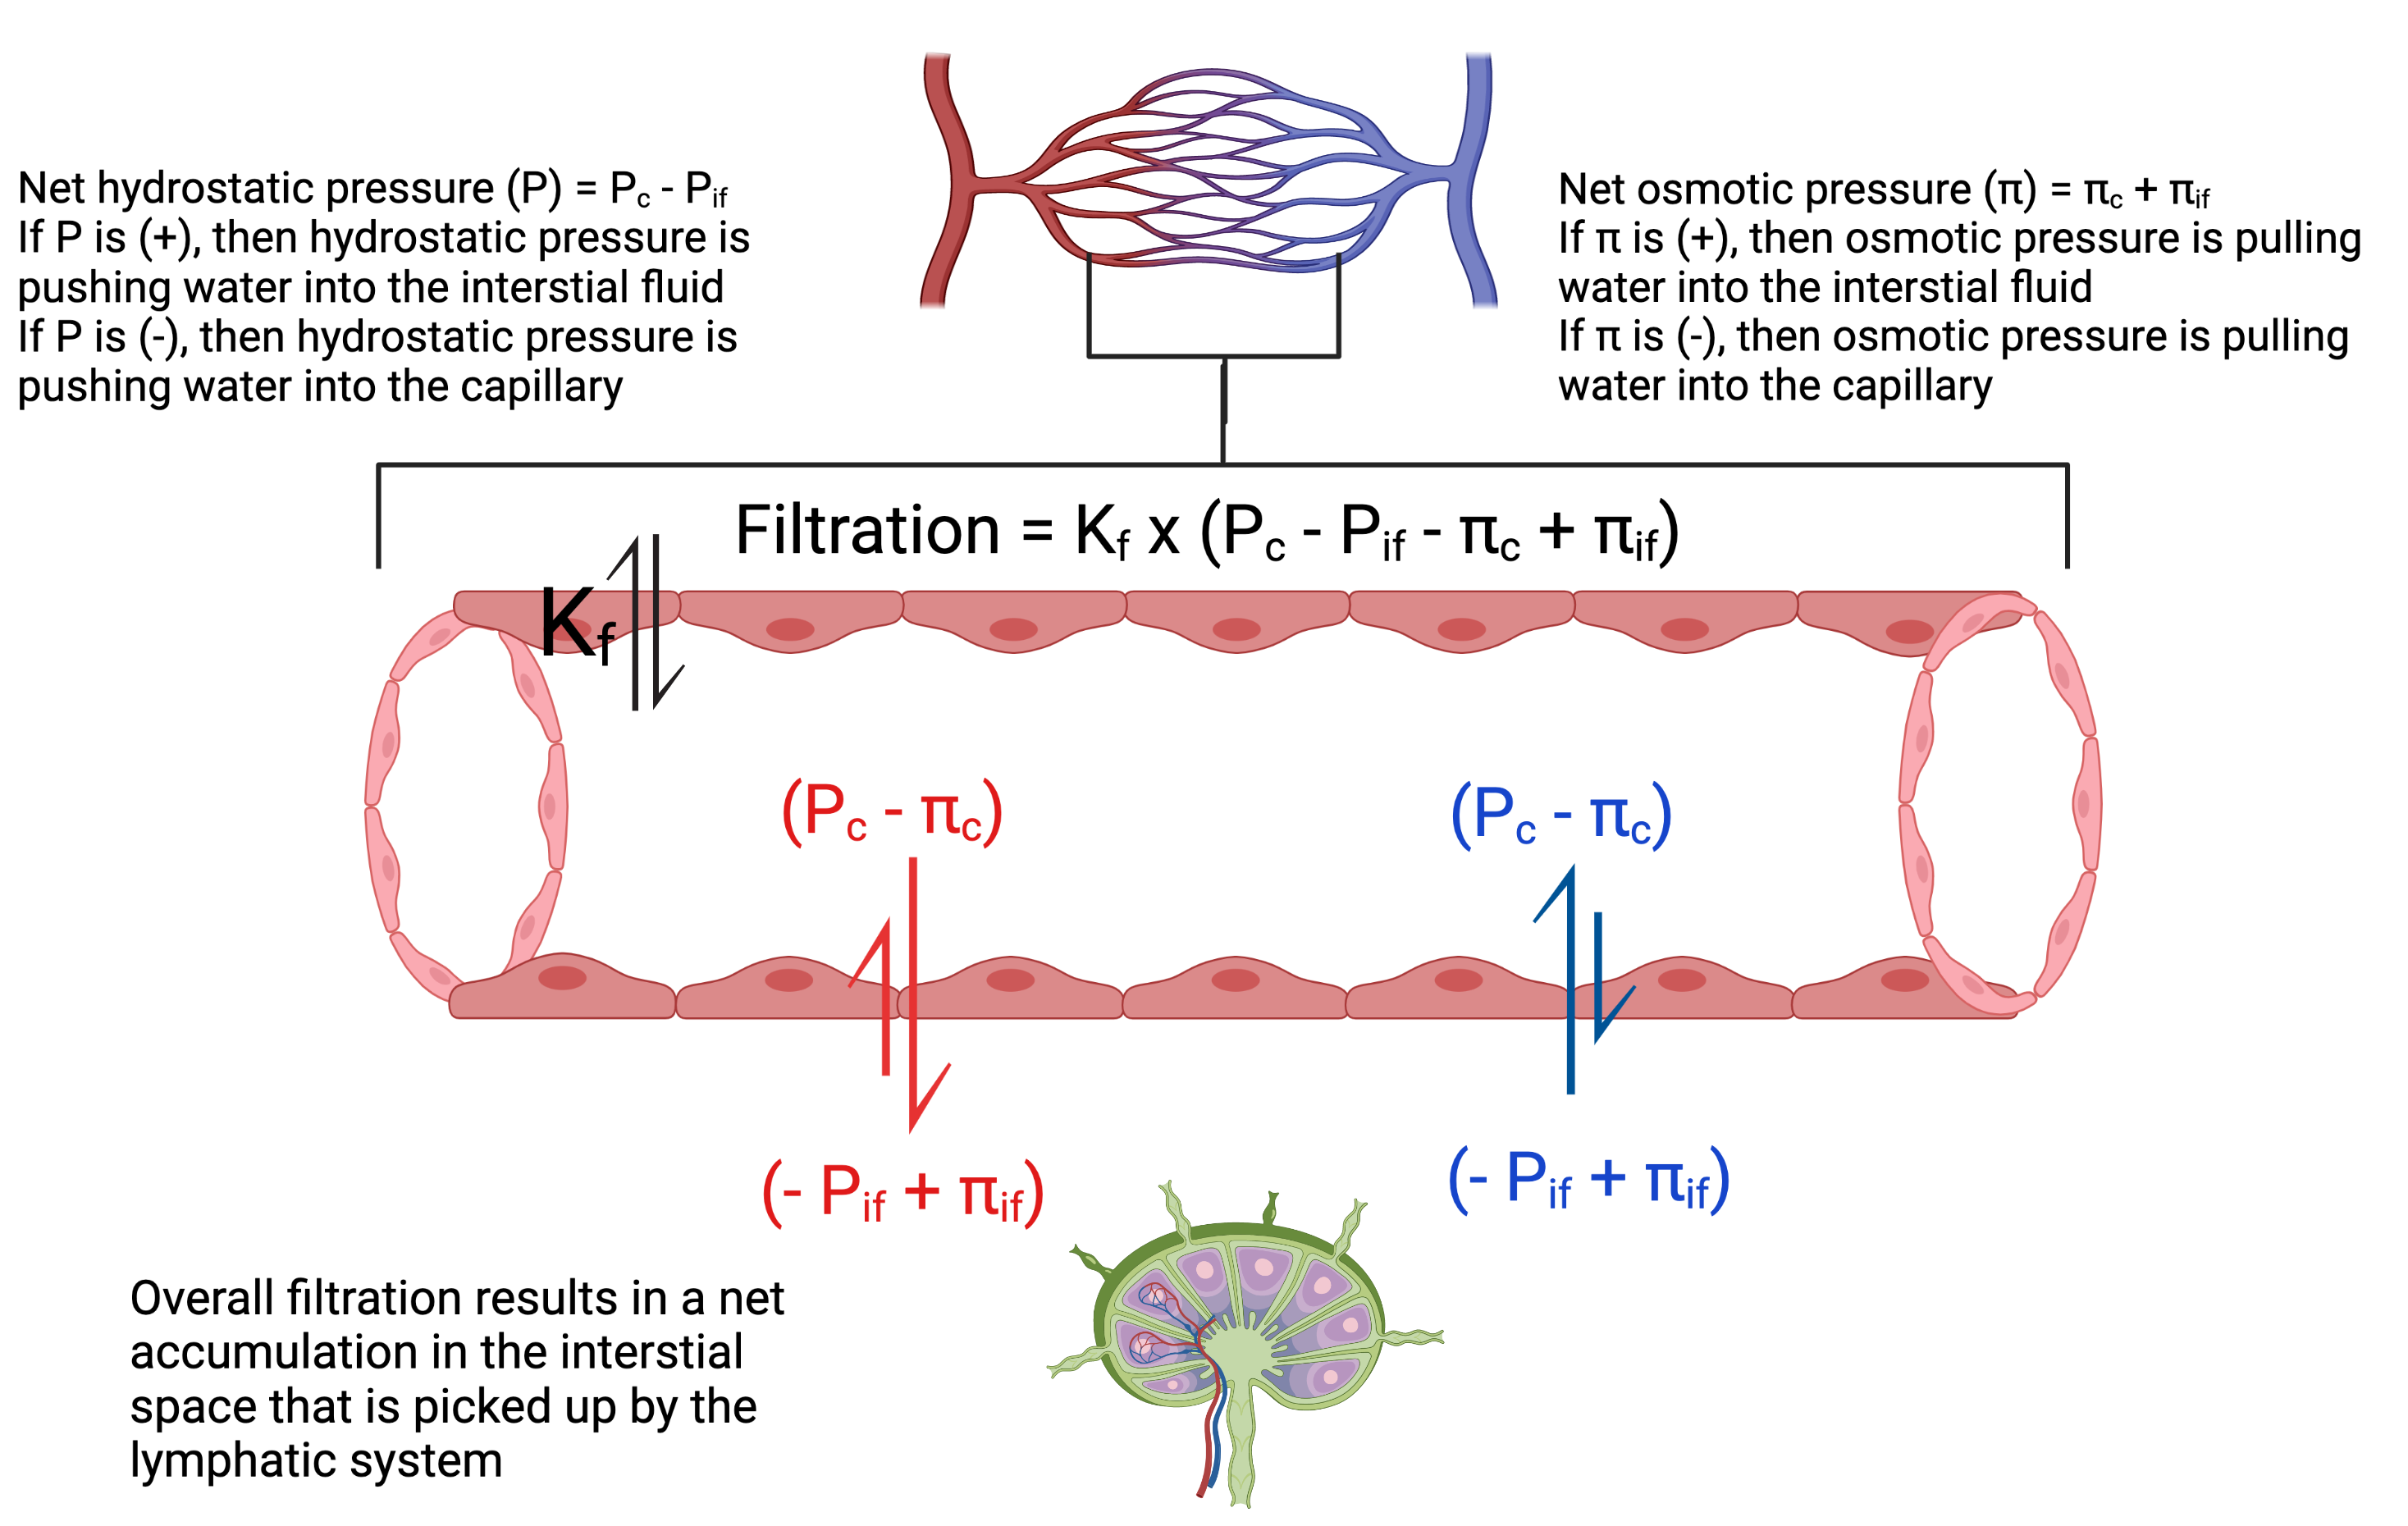
\includegraphics[width=1\linewidth]{./figure/Microcirculation_Regulation.png}
    \caption{Filtration Equation Anatomy \footnotesize{Created with BioRender.com}}
    \label{fig:Microcirculation_Regulation}
\end{figure}

\subsection{Extra Cellular Edema}
Safety factors
Compliance of the tissues is low as long as interstitial fluid hydrostatic pressure is in the negative range
Lymph flow can increase as much as 10- to 50-fold.
“Wash down” of interstitial fluid protein occurs as lymph flow increases (decreased protein concentration in the interstitial fluid reduces the osmotic pressure that tends to pull fluid into the interstitial space AND increase the hydrostatic pressure which also reduces the gradient that tends to push fluid into the interstitial space.


\begin{figure}[!h]
    \centering
    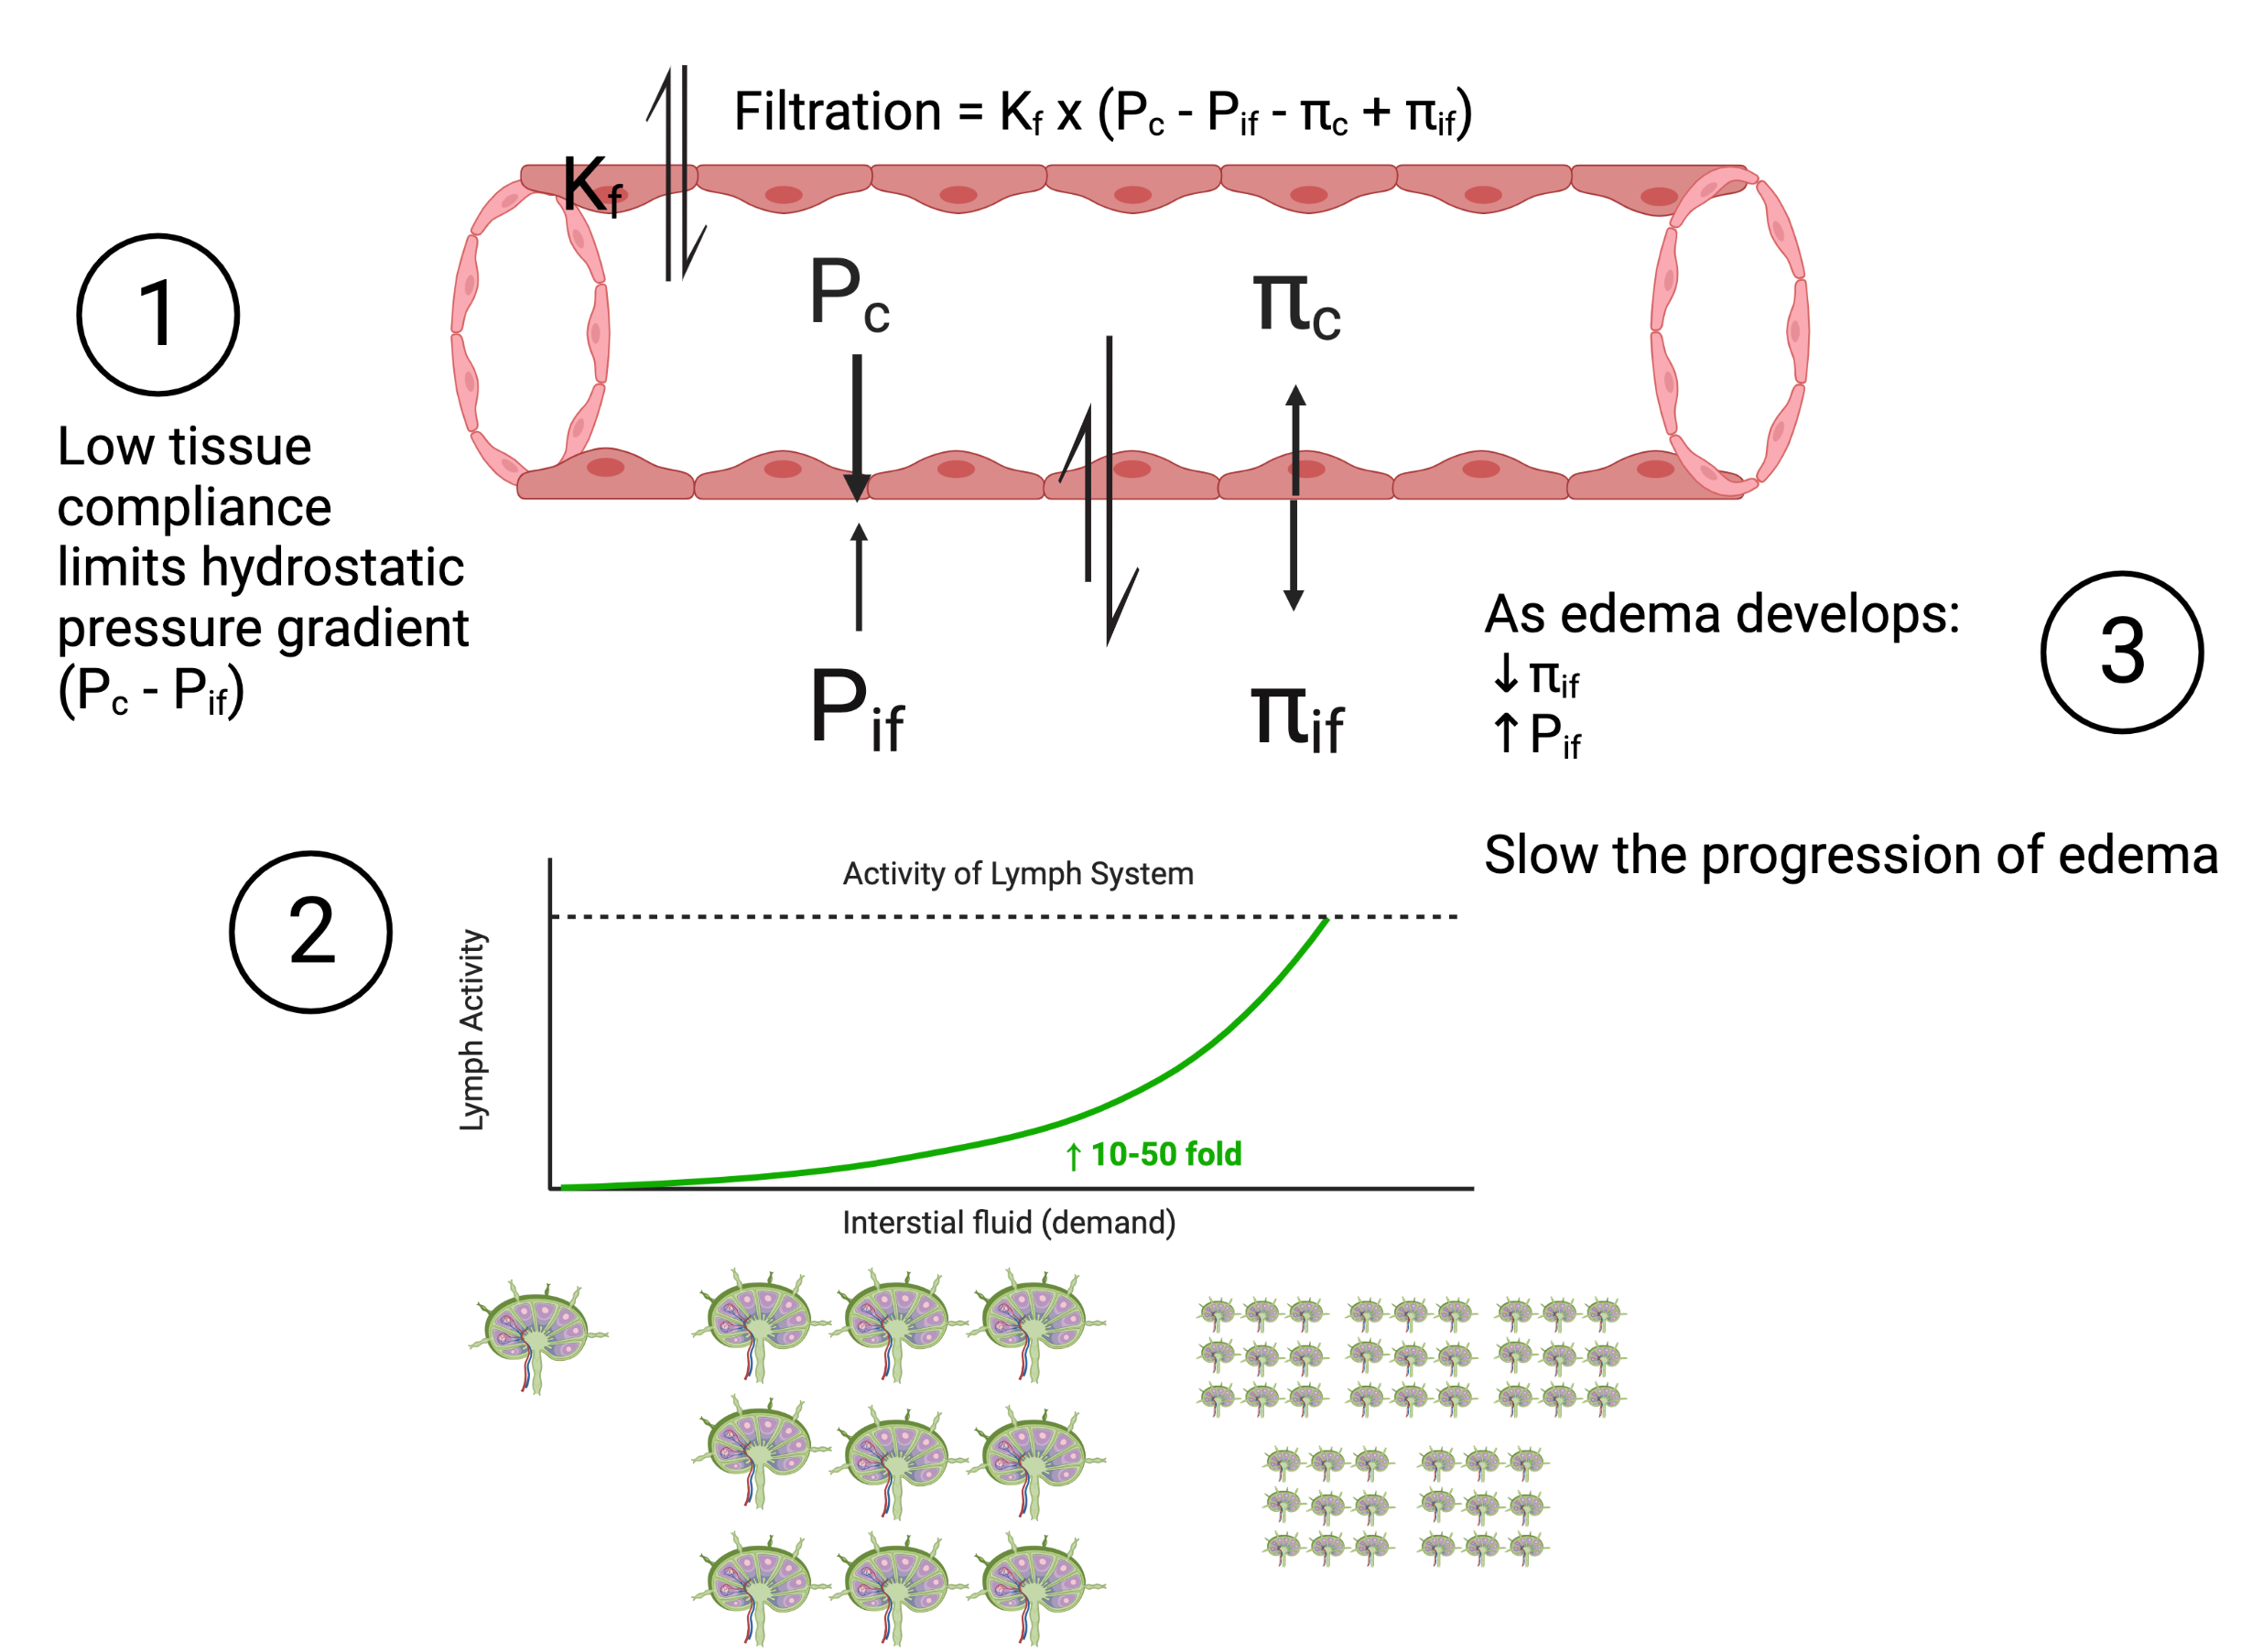
\includegraphics[width=1\linewidth]{./figure/Factors_Prevent_Edema.png}
    \caption{Factors that Prevent Edema \footnotesize{Created with BioRender.com}}
    \label{fig:Factors_Prevent_Edema}
\end{figure}

extracellular edema
Two general causes of extracellular edema are
 (1) abnormal leakage of fluid from the plasma to the interstitial spaces across the capillaries
Increased capillary permeability
Altered hydrostatic pressure
Altered osmotic pressure
(2) failure of the lymphatics to return fluid from the interstitium to the blood, often called lymphedema.

\begin{figure}[!h]
    \centering
    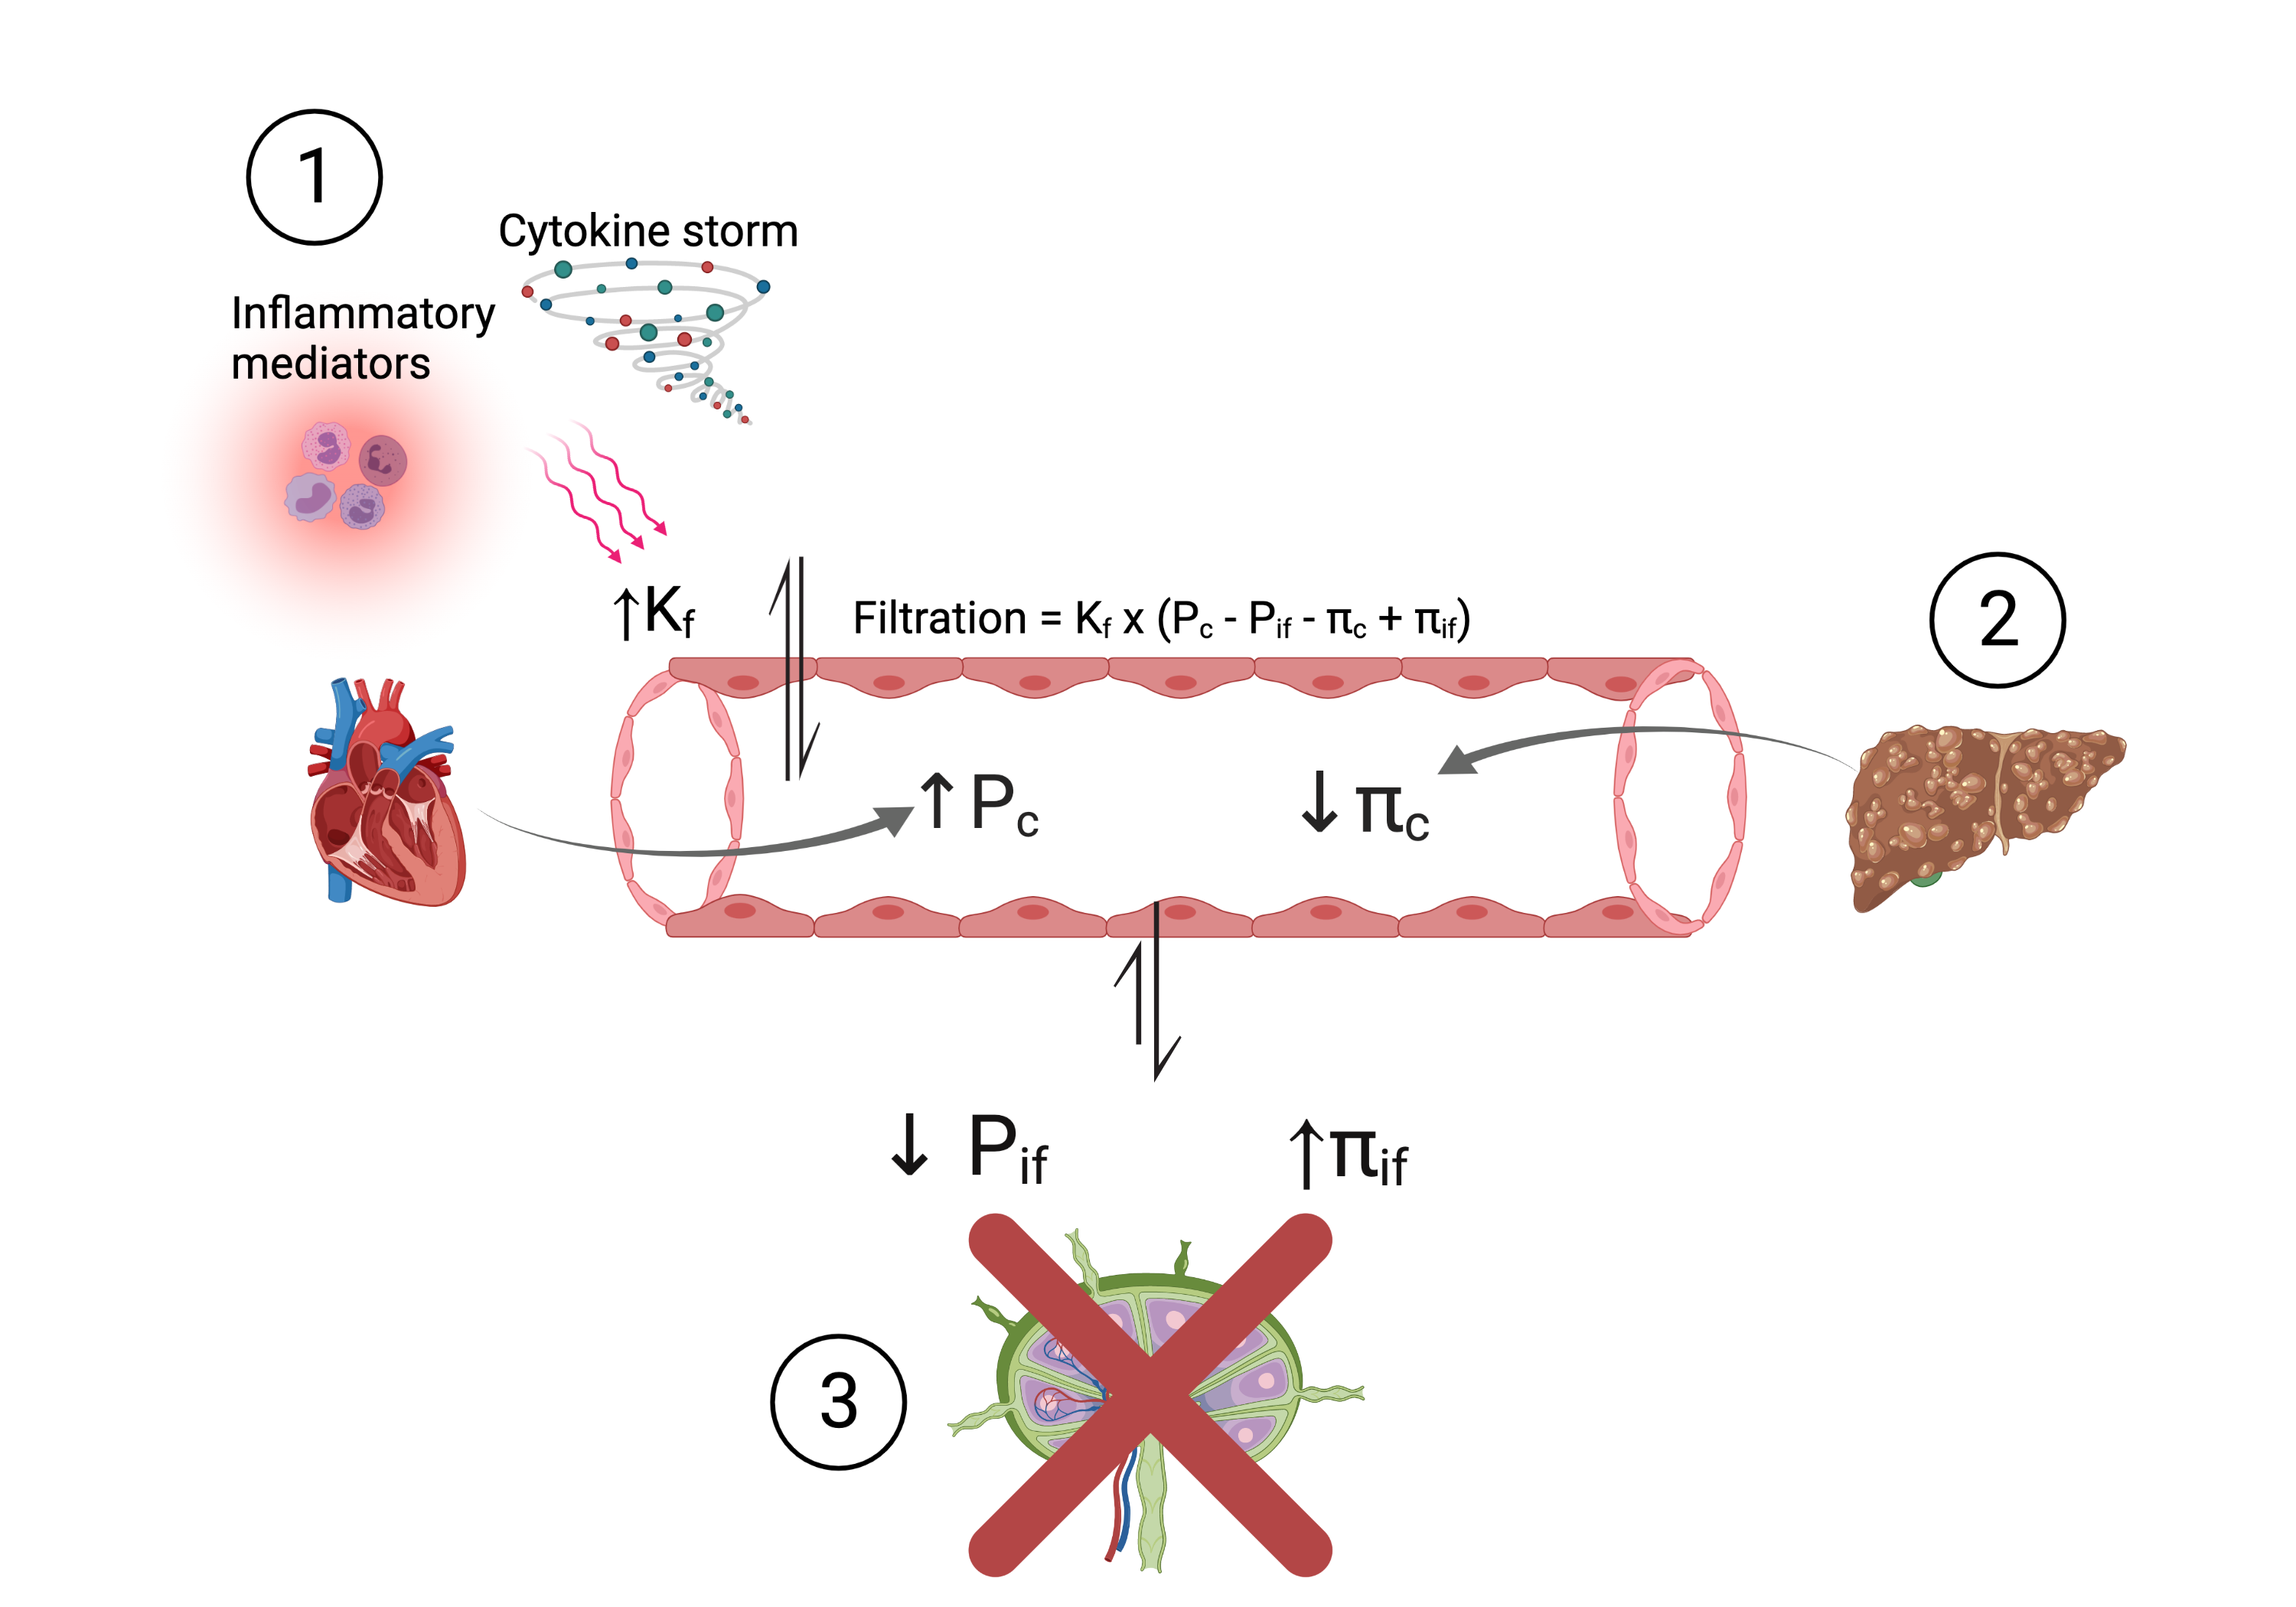
\includegraphics[width=1\linewidth]{./figure/Extracellular_Edema.png}
    \caption{Extra Cellular Edema \footnotesize{Created with BioRender.com}}
    \label{fig:Extracellular_Edema}
\end{figure}

\subsection{Intra Cellular Edema}

There are three conditions that can cause intracellular edema.
\begin{enumerate}
    \item Hyponatremia
    \item Depression of the metabolic systems of the tissues
    \item Lack of adequate nutrition to the cells
\end{enumerate}

Extracellular edema can also cause intracellular edema if the extra cellular edema lowers the ECF osmolarity. Similar to adding a hypotonic solution to the ECF, with reduced ECF osmolarity the ICF osmolarity would pull water into cells until the osmolarity is equalized.

\begin{figure}[!h]
    \centering
    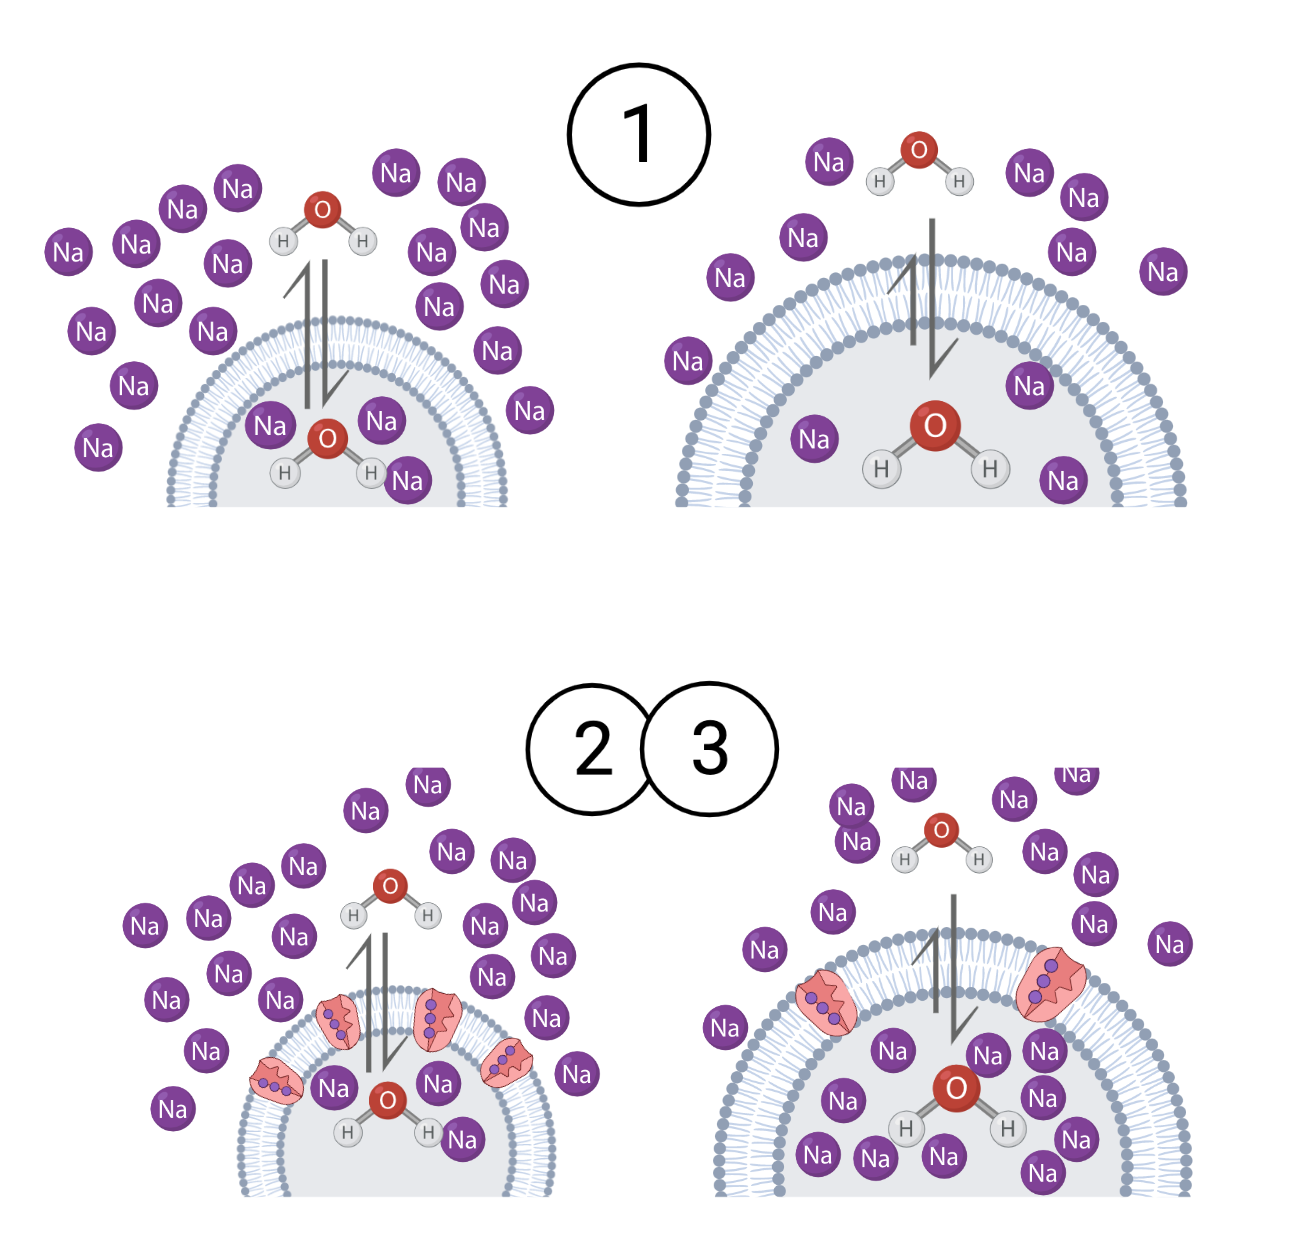
\includegraphics[width=1\linewidth]{./figure/Intracellular_Edema.png}
    \caption{Intra Cellular Edema \footnotesize{Created with BioRender.com}}
    \label{fig:Intracellular_Edema}
\end{figure}

\section{\textit{Clinical Physiology Connections}}

\subsection{Smooth Muscle}

\begin{figure}[!h]
    \centering
    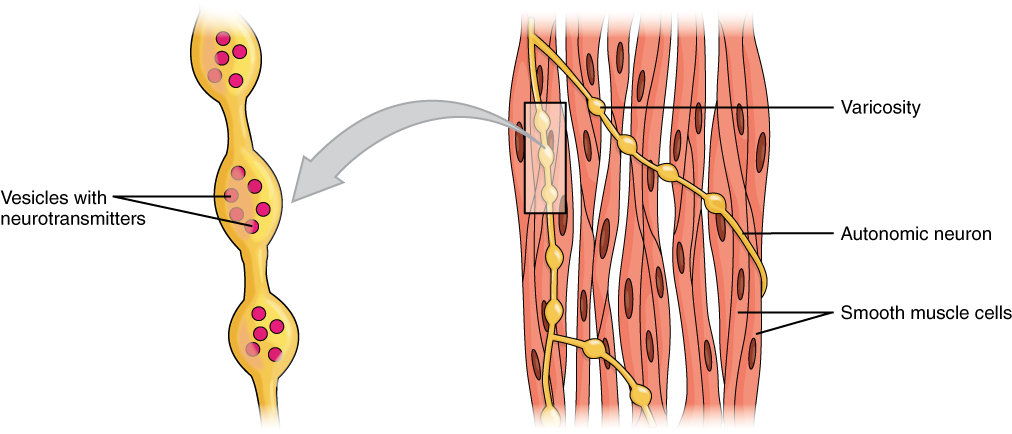
\includegraphics[width=1\linewidth]{./figure/Smooth_Muscle.png}
    \caption{Smooth Muscle \footnotesize{CCBY4.0 from Version 8.25 from the Textbook OpenStax Anatomy and Physiology}}
    \label{fig:Smooth_Muscle}
\end{figure}


\printbibliography[heading=subbibintoc]
